
\section{Selection and Categorisation}\label{sec-selectionandcat}
As described in Chapter~\ref{sec-ATLASDet}, the data collected by ATLAS consists of information measured by various subdetectors. Different processing steps, collectively referred to as \textit{reconstruction}, are applied to unlock physically interpretable objects. This section introduces the specific object recontruction techniques used in the analysis. From this, the event selection, requiring different reconstructed objects to be identified in data and simulations, is then presented as well as the final categorisation separating events into the different regions of the analysis regions.

\subsection{Object Selection}\label{sec-obj}
The ATLAS software supports several object reconstruction techniques. The reconstruction strategies relevant to the \vhbc\ analysis are presented in this section. 

\paragraph{Primary Vertex:} all events considered in the analysis are required to have at least one primary vertex reconstructed from tracks in the \gls{id} \cite{ATL-PHYS-PUB-2015-026}, as detailed in Section~\ref{sec-atlas-lw}.

\paragraph{Electrons:} are reconstructed by matching a deposit in the electromagnetic calorimeter with a track in the \gls{id} \cite{Aaboud:2657964, Aad_2019}, as described in Section~\ref{sec-atlas-el}. Electrons are required to have $p_T > 7$ GeV and $|\eta|<2.47$. They are identified with the \textit{loose} working point of the likelihood discriminant, matching the calorimeter shower shape to an associated track. The $e$ candidates must satisfy $p_T$-dependent isolation criteria in both the \gls{id} and calorimeters. In 1L, the \textit{tight} likelihood identification discriminant is used with stricter calorimeter isolation requirements to better reject the multi-jet background. Additional requirements on the electron selection depend on the lepton channel, as summarised in Table~\ref{tbl:elOb}. $VH$-loose electrons require a loose likelihood identification and are applied in all channels. The $WH$-signal and $ZH$-signal criteria are additionally applied in the 1L and 2L channels respectively, with a higher $p_T$ threshold due to the triggers. 

\begin{table}[!htbp]
  \begin{center}
    \resizebox{0.9\textwidth}{!}{
      \begin{tabular}{ccccccc} \hline \hline
        Selection & $p_T$ & $\eta$ & ID & $d_{0}^{\mathrm sig}$ &  $|\Delta{z_{0}}\sin\theta|$ & Isolation \\ \hline
        $VH$-loose & $>$7 GeV & $|\eta|< 2.47$ & \textit{Loose} & $ <5$ & $<0.5$ mm & Loose \\ % Loose\_VarRad
        $ZH$-signal & $>$27 GeV & $|\eta|< 2.47$ & \multicolumn{3}{c}{Same as $VH$-loose} \\
        $WH$-signal & \multicolumn{2}{c}{Same as $ZH$-signal} & \textit{Tight} & \multicolumn{2}{c}{Same as $ZH$-signal} & Strict \\ %HighPtCaloOnly
        \hline\hline
      \end{tabular}
    }
    \caption{Electron selection requirements. $ZH$-signal and $WH$-signal are abbreviated as $VH$-signal in the text.} 
    \label{tbl:elOb}
  \end{center}
\end{table}

\paragraph{Muons:} are reconstructed by matching an energy deposit in the \gls{ms} with information from the \gls{id} \cite{Aad:2746302}, as detailed in Section~\ref{sec-atlas-mu}. They are required to have $p_T >$ 7 GeV, $|\eta| < 2.7$, to satisfy the \textit{loose} identification criterion, and be isolated in the \gls{id} according to $p_T$-dependant criteria. These requirements are summarised in Table~\ref{tbl:muonOb} and vary depending on the lepton channel similarly to the electron requirements. The $VH$-loose requirements are applied to muons in all channels. The $WH$-signal and $ZH$-signal are additionally applied to the 1L and 2L channels respectively, with a \textit{medium} identification likelihood criterion and a strict track-based isolation used in 1L to suppress the multi-jet background.

\begin{table}[!htbp]
    \begin{center}
      %\resizebox{\textwidth}{!}{
        \begin{tabular}{ccccccc} \hline \hline
          Selection & $p_T$ & $\eta$ & ID & $d_{0}^{\mathrm sig}$  & $|\Delta{z_{0}}\sin\theta|$ & Isolation \\ \hline
          $VH$-loose & $>$7 GeV & $|\eta|< 2.7$ & Loose & $ <3$ & $<0.5$ mm & Loose \\ % Loose\_VarRad
          $ZH$-signal & $>$27 GeV & $|\eta| < 2.5$ & \multicolumn{4}{c}{Same as $VH$-loose} \\
          %WH-signal & $>$25 GeV ($>$27 when $p_T^V<$ 150 GeV) & $|\eta|< 2.5$ & Medium quality & $ <3$ & $<0.5$ mm & HighPtTrackOnly \\
          $WH$-signal & \makecell[c]{$>$25 GeV if $p_T^V>$ 150 GeV\\ $>$27 GeV if $p_T^V<$ 150 GeV} & $|\eta|< 2.5$ & Medium & $ <3$ & $<0.5$ mm & Strict \\
          \hline\hline
        \end{tabular}
      %}
      \caption{Muon selection requirements. $ZH$-signal and $WH$-signal are abbreviated as $VH$-signal in the text.} 
      \label{tbl:muonOb}
    \end{center}
  \end{table}
  
\paragraph{Taus:} hadronically decaying $\tau$-leptons are identified and vetoed in 1L using an \gls{rnn}-based tagger \cite{ATL-PHYS-PUB-2019-033}, as presented in Section~\ref{sec-atlas-tau}. Taus are required to have a $p_T >$ 20 GeV, $|\eta| <$ 2.5, and to have 1 or 3 associated tracks. In 0L and 2L, if the jet passes a \textit{loose} working point requirement for hadronically decaying $\tau$-lepton identification, it is no longer considered a jet and cannot be considered as a candidate for the reconstruction of the Higgs boson. 

\paragraph{Missing Transverse Energy:} as described in Section~\ref{sec-atlas-met}, neutrinos are not detectable in ATLAS and their presence is inferred from momentum imbalance in the transverse plane. \etm\ is calculated as the negative vectorial sum of the transverse momentum of physics objects (electrons, muons, hadronic $\tau$, and jets), with an additional track-based \textit{soft term} from unassigned good-quality tracks \cite{ATLASmetReco}. 

\paragraph{Jets} Three types of jets introduced in Section~\ref{sec-atlas-jets} are used in the analysis, all reconstructed with the anti-$k_t$ algorithm \cite{Cacciari:2008gp}:
\begin{enumerate}
  \item \textit{Small-$R$ jets}: are reconstructed from topological clusters of energy deposits in the hadronic calorimeter based on the reconstructed PFlow objects with a radius $R = 0.4$. A jet is considered as \textit{central} if $|\eta| < 2.5$ and $p_T$ > 20 GeV, and as \textit{forward} if 2.5 $\leq |\eta|$ < 4.5 and $p_T > 30$ GeV. Central (forward) jets with a $p_T < 60$ GeV ($p_T < 120$ GeV) are required to originate for the primary vertex as identified by the \glsreset{jvt}\gls{jvt} to limit the pile-up background \cite{atlasPUJVT}. \textit{Tight} jet cleaning criteria are applied to suppress non-collision background. Central jets are used in the resolved regime to reconstruct the Higgs candidate with flavour tagging. 
  \item \textit{Large-$R$ jets}: similar to small-$R$ jets with a larger radius $R = 1.0$, they are required to have $p_T > 250$ GeV and $|\eta| < 2$, and are used in the boosted regime to reconstruct the Higgs candidate. 
  \item \textit{Variable-$R$ (\gls{vr}) track-jets}: are reconstructed with a $p_T$-dependent radius optimised for double $b$-tagging of the boosted $H \rightarrow b\bar{b}$ decay \cite{ATL-PHYS-PUB-2017-010}. They must have $p_T > 10$ GeV and $|\eta| < 2.5$. These track-jets are used to reconstruct the $b$-tagged objects inside the large-$R$ jet. 
\end{enumerate}
As outlined in Section~\ref{sec-atlas-jets}, jets benefit from extensive corrections and calibrations to improve their reconstructed mass, energy, and axis direction.

\paragraph{Flavour Tagging} Jet flavour tagging is perhaps the most important part of the event reconstruction. The latest available \gls{dl1r} tagger from Run 2 is used for both $b$- and $c$-tagging in the resolved and boosted regime \cite{atlas:FTAGRUN2}. The methodology differs slightly between the two regimes of the analysis due to the different flavour tagging needs.
\begin{itemize}[leftmargin=*]
\item In the resolved regime, \gls{dl1r} is used to tag both $b$- and $c$-jets. The so-called \textit{\glsreset{pcft} \gls{pcft} scheme}, illustrated in Figure~\ref{fig:pseudotag}, is deployed to allow for a coherent joint definition and simultaneous calibration of $b$- and $c$-tagged jets, adopting the technique first introduced for 2D $c$-tagging in the \vhc\ analysis \cite{Collaboration:2721696}. The \gls{dl1r} tagger assigns a $b$-tagging and a $c$-tagging discriminant scores\footnote{With flavour fractions set as ${f^b}_c = 0.018$ and ${f^c}_b = 0.3$, respectively.} from Equations \ref{bdisc} and \ref{cdisc} to selected central jets. To tag a jet, the associated score must be higher than a specific cutoff value defining a \glsreset{wp}\gls{wp} selection efficiency. Jets can be assigned one of 5 possible labels based on 2 $b$-tagging and 2 $c$-tagging \glspl{wp}, as outlined in Figure~\ref{fig:pseudotag}. These \glspl{wp} are tested in a strict successive order, with first a 60\% \textit{tight} $b$-tagging point (bin 4) followed by a \textit{looser} 70\% $b$-tagging \gls{wp} (bin 3). A jet passing these selections is labelled $B$\footnote{The distinction of this two $b$-tagged bins is relevant for the \glspl{mva} of the analysis}. Otherwise, it is considered for $c$-tagging with first a \textit{tight} working point at 25\% efficiency (bin 2), followed by a \textit{loose} \gls{wp} at an exclusive efficiency of 20\% (bin 1) - so that 45\% of the $c$-jets are effectively selected in the combined tight and loose bins. A jet selected by the tight $c$-tagging \gls{wp} is labelled $T$, and $L$ if it only passes the loose \gls{wp}. A jet failing to pass any tagging selection is not tagged and labelled $N$ (bin 0). The $b$-tagging \glspl{wp} correspond to official ATLAS ones for \gls{dl1r} \cite{atlas:FTAGRUN2}, while those for $c$-tagging are optimised for the purpose of this analysis. The tagging efficiency of each bin is displayed in Figure~\ref{fig:pseudotag}, as measured in a \textsc{Powheg}+\textsc{Pythia} 8 sample of semi-leptonic \ttb\ events. The calibration of the five bins is performed simultaneously for the analysis following the methodology described in Ref. \cite{atlas:FTAGRUN2}.%, with some results presented in Appendix \ref{appsec-vh-ftagcal}.

\begin{comment}
\begin{table}[h!]
  \begin{center}
      \begin{tabular}{c|c|cccc}
        \hline \hline
        \multirow{2}{*}{PCFT bin} & \multirow{2}{*}{PCFT bin name} & \multicolumn{4}{c}{Jet tagging efficiency $\epsilon_{jet}$}\\
        & & $b$-jet &  $c$-jet &  light-jet & $\tau$-jet \\ 
        \hline
        1 & $c$-loose & 11.5\% & 20.5\% & 6.5\%   & 18.5\%\\
        2 & $c$-tight & 4.8\%  & 24.2\% & 0.9\%   & 19.5\%\\
        3 & $b$-70\%  & 11.2\% &  5.2\% & 0.13\%  &  1.7\%\\
        4 & $b$-60\%  & 58\%   & 2.65\% & 0.051\% & 0.49\%\\
        \hline \hline
      \end{tabular}
    \caption{Jet tagging efficiencies for $b$-, $c$-, light- and $\tau$-jets in the \gls{pcft} scheme, measured in a \textsc{Powheg}+\textsc{Pythia} 8 sample of semi-leptonic \ttb\ events.}
    \label{tbl:PCFTtageff} % Don't understand why thigh is not at 20\%
  \end{center}
\end{table}
\end{comment}
\begin{figure}[h!]
  \center
    \begin{minipage}[c]{0.65\textwidth}
      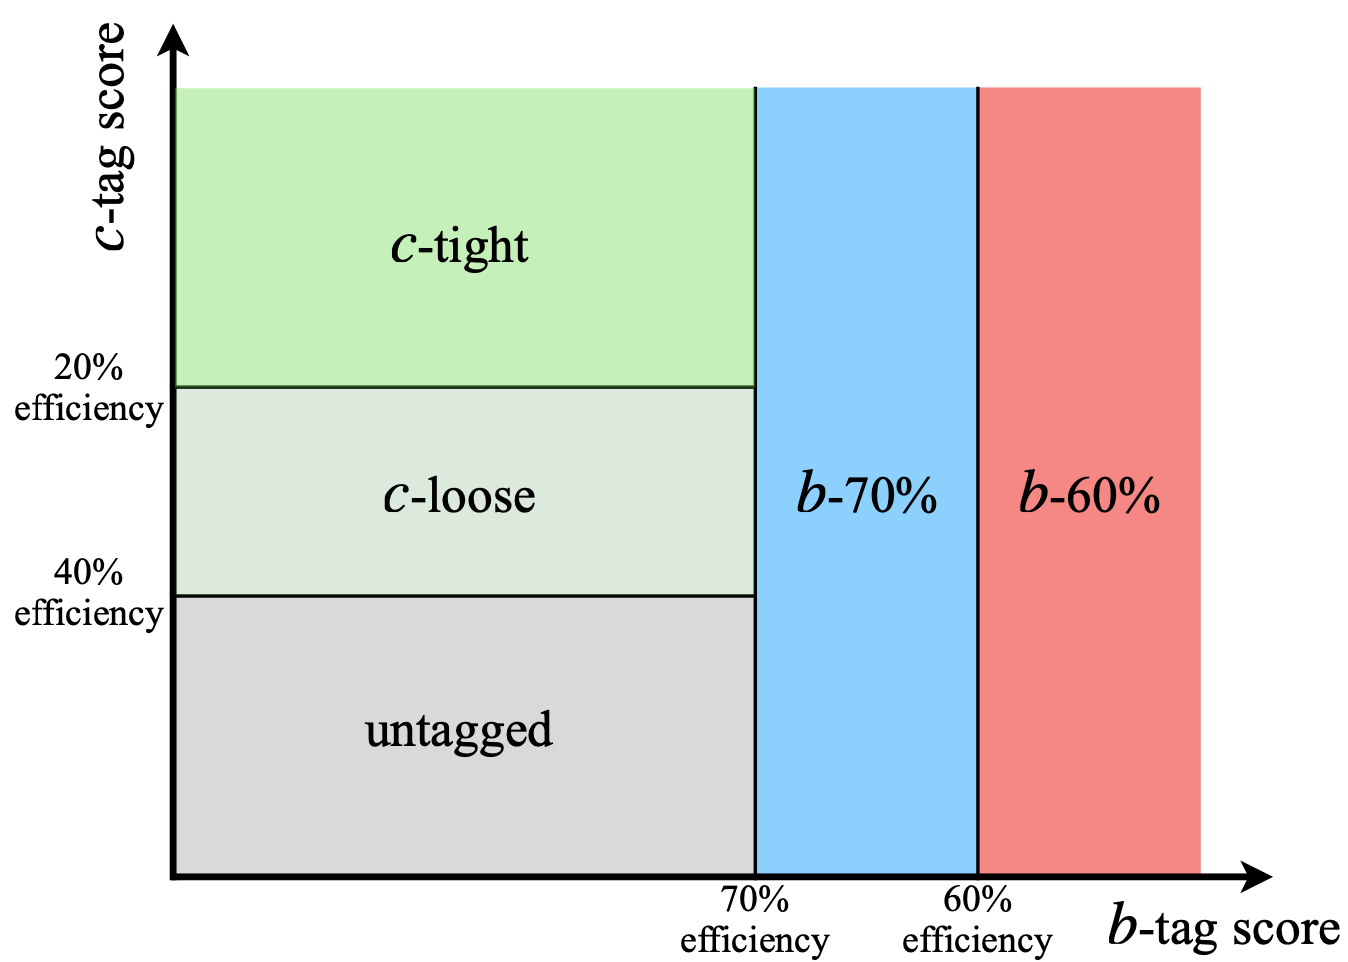
\includegraphics[width=0.98\textwidth]{Images/VH/pseudocontinuous.png}
    \end{minipage}
    \begin{minipage}[c]{0.34\textwidth}
      \caption{The pseudo-continuous flavour tagging scheme defining simultaneously 2 $b$-tagged, a tight $c$-tagged, a loose $c$-tagged, and a non-tagged bins. The jet tagging efficiencies for $b$-, $c$-, and light-jets in the \gls{pcft} scheme are displayed for each region.} 
      \label{fig:pseudotag}
    \end{minipage}
\end{figure}

\item The boosted regime only targets $b$-jets, with the single-jet \gls{dl1r} tagger used. As such, the standard pseudo-continuous $b$-tagging method is used \cite{atlas:FTAGRUN2}. The track-jets associated with the leading large-$R$ jet are given a $b$-tagging score based on the per-flavour probabilities predicted by \gls{dl1r}. The 85\% working point is adopted to maximise the signal yield, due to the statistical limitations in the boosted regime. Track-jets passing this working point are $B$-tagged, otherwise, they are untagged $N$. The official calibration from Ref. \cite{atlas:FTAGRUN2} is used and extended to higher $p_T$ with uncertainty extrapolation due to the large range of $p_T$ probed in the analysis \cite{cjettaggingCalib, ATLAS:2023lwk}.
\end{itemize}
The superior single-jet \gls{gnn} taggers introduced in Chapter \ref{chap-ftag} or the boosted decay tagger GN2X \cite{ATL-PHYS-PUB-2023-021} presented in Appendix~\ref{app-chap-GN2X} were not available during the analysis, and their calibration is, at the time of writing, still ongoing. Leveraging the improvements of these \gls{gn2}-based taggers represents an exciting avenue of progress for future iterations of this study, for both the resolved and boosted regimes. 

\paragraph{Object Overlap:} this procedure is applied to avoid double-counting electrons, muons, small-$R$ and large-$R$ jets, and hadronic $\tau$-leptons passing the object selection.

\subsection{Event Selection}\label{sec-regimeCat}
A subset of all ATLAS recorded events during Run 2 is selected for the analysis based on specific triggers. The trigger selections of \vhb\ and \vhc\ are harmonised for the combined analysis, and specified per lepton channel. In 0L, the lowest un-prescaled \etm\ trigger is used with an increasing lower threshold rising from 70 GeV for data recorded in 2015, 90 to 110 GeV for 2016, and to 110 GeV for 2017 and 2018 due to higher trigger rate later in Run 2. The 1L channel triggers cover both the $e$ and the $\mu$ subchannels. The lowest un-prescaled single-electron trigger is deployed for the $e$-channel. For muons, the \etm\ trigger of 0L is applied for events with \ptv\ > 150 GeV, while the lowest un-prescaled single-muon trigger is used at lower \ptv. Finally, the triggers for 2L are equivalent to 1L except for the muon channel where the \ptv\ threshold for switching between triggers is raised to 250 GeV. The use of \etm\ trigger at high \ptv\ for muons increases the signal acceptance by approximately 5\%. For leptonic triggers, reconstructed leptons in the event are required to match the triggered leptons. \\ 

The different regimes of the analysis are defined by flavour tagging and the strategy to reconstruct the Higgs boson. In the resolved regime, an event must have at least two central jets. Two candidate jets are selected to reconstruct the Higgs using the so-called \textit{All Signal Jets} strategy, and define an event tag by combining their individual tags. A tag hierarchy is introduced, following the rank ordering: $B$ > $T$ > $L$ > $N$. The pair of candidates is selected from the two central jets having the highest ranked tags, or the highest $p_T$ in case of ties. Events are labelled based on the tag of the selected jets, e.g., $TT$ is assigned to events with 2 tight $c$-tagged jets and no $b$-jet, and $BL$ to events with a $b$-tagged and a loose $c$-tagged jets. In the boosted regime, at least 2 track-jets are required to be associated with the large-$R$ jet leading by $p_T$, and the tags of at most 3 associated track-jets with the highest $p_T$ are considered in each event. This labelling and the reconstructed \ptv\ define the different regimes of the resolved and boosted \vhb\ and \vhc\ parts of the combined analysis. Each regime is applied specific selections to reconstruct the Higgs candidates. 

\paragraph{Resolved Higgs candidates:} for \vhb, the two candidates must be $B$-tagged (\gls{pcft} bins 3 or 4) with no additional $b$- nor tight $c$-tagged jets allowed\footnote{In 2L, additional $T$-tagged jets are permitted due to the low statistics and the different derivation of the top CR.}, while in \vhc\ no $B$-tagged jet is allowed and at least one of the candidates must be tight $c$-tagged ($T$). As detailed in the next section, two types of \glspl{cr} are defined orthogonally to the \glspl{sr} by changing this flavour selection: the top \glspl{cr}, combining at least 1 $B$-tag with at least 1 $T$-tag, and the $V+l$ \glspl{cr} requiring 1 loose $c$-tagged jet ($L$) with an untagged ($N$) jet for \vhc. The Higgs candidates are sorted by $p_T$ into a leading $j_1$ and subleading $j_2$ candidate. The leading candidate must have $p_T > 45$ GeV, while other jets are required to have $p_T > 20$ GeV. The invariant mass of the Higgs candidate $m_{bb}$ ($m_{cc}$) must be above 50 GeV before applying energy corrections, to avoid low-mass $V$+jets gluon splitting mismodelling.  

\paragraph{Boosted Higgs candidates:} the selection requires exactly 2 $B$-tags among the 3 track-jets leading by $p_T$ associated to the leading large-$R$ jet. The reconstructed mass of the Higgs candidate based on the leading-$R$ jet mass $m_J$ must satisfy $m_J > 50$ GeV, with a leading large-$R$ jet $p_T > 250$ GeV. \\

The small overlap between the boosted \vhb\ and resolved \vhc\ selected events is found to be negligible. In all regimes, the number of reconstructed charged lepton in the final state defines three channels as the 0-lepton (0L), 1-lepton (1L), and 2-lepton (2L). The objective of this leptonic selection is to reconstruct the associated $V$ boson. The selection of events in the resolved regime is presented in Table~\ref{tbl:VHbbccevSelTable}, and Table~\ref{tbl:VHbbBoostevSelTable} for the boosted regime. Additional channel-specific requirements are also introduced to limit background contamination. They are reviewed in the next section.

\subsubsection{Selection specific to the 0-lepton channel}\label{subsubsec-0Lsel}
In 0L, no $VH$-loose lepton is allowed and \etm\ should be $>$ 150 GeV ($>$ 250 GeV) in the resolved (boosted) regime, to identify the decay $Z \rightarrow \nu\nu$. Additionally, in the resolved regime the scalar sum $S_T$ of the jet $p_T$ in the events must be $> 120$ GeV ($> 150$ GeV) for 2-jet ($\geq$ 3 jets) events to avoid a mismodelled region in simulation due to the triggers. In a decay of a $W \rightarrow \tau \nu$ followed by a hadronic decay of the $\tau$-lepton reconstructed as a jet, there are no electrons nor muons in the final state. To limit this $\tau$-contamination in the 0L channel, an extra selection is applied in the resolved regime if at least 1 hadronic $\tau$ is reconstructed. The transverse $W$ mass \[ m_T^W = \sqrt{2 p_T^l E_T^{\textrm{miss}} (1 - \cos(\Delta \phi(l, E_T^{\textrm{miss}} ) ) ) } \] is required to be $m_T^W \geq$ 10 GeV, with the $W$ boson $p_T$ estimated from the vectorial sum of the leading hadronic $\tau$ momentum ($p_T^l$) and \etm\ instead of \ptv. To limit the multi-jet background, so-called \textit{anti-QCD cuts} are also applied in all regimes:
\begin{itemize}
    \item The azimuthal angle between \etm\ and the $H$ must satisfy $|\Delta \phi(E_t^{\textrm{miss}}, H)| > 120 \ensuremath{^\circ}$.
    \item The minimum azimuthal angle between \etm\ and the jets must be $> 20\ensuremath{^\circ}$ ($> 30 \ensuremath{^\circ}$) for resolved 2-jet (3-jet) events and $> 30\ensuremath{^\circ}$ for the boosted regime.
    \item In resolved only, the azimuthal angle between the candidate jets must satisfy $|\Delta \phi(j_1, j_2)| < 140 \ensuremath{^\circ}$.
\end{itemize}
The cuts are tuned to limit the multi-jet contamination to a fraction of order 1\% of the total background in 0L, making this background negligible in the 0-lepton channel. 

\subsubsection{Selection specific to the 1-lepton channel}
In the 1L channel, the targeted vector boson decay is a $W \rightarrow \ell\nu$, with $\ell = e, \mu$. Exactly 1 $WH$-signal lepton is required, with events having more than 1 $VH$-loose lepton vetoed\footnote{The first $VH$-loose lepton corresponds to the $WH$-signal lepton.}. The vector boson is reconstructed from the vectorial sum of the \etm\ and the lepton transverse momentum $p_T^l$, with \ptv\ $> 75$ GeV. To suppress the multi-jet background, events with one electron are required to have an \etm\ $>$ 30 GeV ($> 50$ GeV) in the resolved (boosted) regime, with a reconstructed $m_T^W > 20$ GeV for events with transverse momentum $p_T^V$ below 150 GeV. For the resolved $\mu$-channel, as the same \etm\ trigger is used as in the 0L, the scalar sum of $p_T$ is similarly constrained with $S_T > 120$ GeV ($> 150$ GeV) for 2-jet ($\geq$ 3 jets) events. A significant background in the 1-lepton channel is the \ttb\ production, with both $t$-quarks decaying into a $W$ boson and a $b$-quark. Events where one of the $W$ boson decay follows $W \rightarrow \tau \nu$, with the $\tau$ decaying hadronically, and the other $W$ decays into an $e$ or a $\mu$ have the same leptonic signature as the signal. A strict hadronic $\tau$-veto is applied in all regimes to suppress this background. Events passing the 0-lepton selection with $\geq 1$ hadronic taus are moved to the 1-lepton channel with the leading hadronic $\tau$ used similarly to any other lepton, $e$ or $\mu$. The migration recovers $\sim$ 10\% ($\sim$ 20\%) of $WH$ signal where $W\rightarrow \tau \nu$ and the $\tau$-lepton decays hadronically in the resolved (boosted) regime. This technique helps decorrelating the $WH$ and $ZH$ measurements in the \vhb\ side.

\subsubsection{Selection specific to the 2-lepton channel}
The 2L channel targets the $Z \rightarrow\ell\ell$ bosonic decay, with the $Z$ reconstructed from two loosely identified leptons of the same flavour ($VH$-loose). At least one lepton must pass the $ZH$-signal lepton requirements. In the di-muon channel, the leptons are further required to be of opposite charges\footnote{This is not applied to the di-electron channel due to a significantly higher charge misidentification.}. To suppress non-resonant lepton-pair from the \ttb\ and multi-jet backgrounds, the invariant mass of the di-lepton system is required to be consistent with the $Z$ mass, with $81 < m_{\ell\ell} < 101$ GeV in the resolved and $66 < m_{\ell\ell} < 111$ GeV in the boosted regime. The leptons must satisfy $p_T > 25$ GeV, with a stricter $p_T > 27$ GeV required for the leading muon when the event is selected by the muon trigger.\\


\begin{table}[htbp]
  \resizebox{1\textwidth}{!}
  {
  \renewcommand*{\arraystretch}{1.1}
  \begin{tabular}{C{3.3cm}|C{2.8cm}|C{2.5cm}|C{1.8cm}|C{2.5cm}|C{1.8cm}}
  \hline \hline
  \textbf{Selection} & \textbf{0-Lepton} & \multicolumn{2}{c|}{\textbf{1-Lepton}} & \multicolumn{2}{c}{\textbf{2-Lepton}}  \\
  & & $e$-channel & $\mu$-channel & $e$-channel & $\mu$-channel \\ \hline \hline
  Trigger & \etm\ & Single-electron & \etm\ & Single-electron & \etm\ \\
  Leptons & 0 $VH$-loose lepton & \multicolumn{2}{c|}{1 $WH$-signal lepton} & \multicolumn{2}{c}{$\geq$ 1 $ZH$-signal lepton} \\
   & & \multicolumn{2}{c|}{No second $VH$-loose lepton} & \multicolumn{2}{c}{2 $VH$-loose leptons} \\
   &  & \multicolumn{2}{c|}{No hadronic $\tau$} & \multicolumn{2}{c}{Same flavour leptons} \\
   &  &  \multicolumn{2}{c|}{} & \multicolumn{2}{c}{Opposite charge for $\mu\mu$} \\ \hline
  \ptv\ &  \multicolumn{5}{c}{$>$ 400 GeV} \\
  Large-$R$ jet & \multicolumn{5}{c}{$\geq$ 1 large-$R$ jet ($R$ = 1.0), $p_T >$ 250 GeV, $|\eta| < 2$} \\
  Track-Jets & \multicolumn{5}{c}{$\geq$ 2 track-jets ($p_T > 10$ GeV, $|\eta| < 2.5$) matched to the leading large-$R$ jet} \\
  Tagging & \multicolumn{5}{c}{Exactly 2 of the 3 leading track-jets matched to the large-$R$ jet must be $b$-tagged} \\
  $m_J$ & \multicolumn{5}{c}{$> 50$ GeV} \\ \hline
  \etm\ & $>$ 200 GeV & $>$ 50 GeV & - & \multicolumn{2}{c}{-} \\ % WARNING For 0L, it's 200 in the text but 250 in the table
  $|\Delta\phi(E_T^{\textrm{miss}}, H)|$ & $> 120\ensuremath{^\circ}$ & \multicolumn{2}{c|}{-} & \multicolumn{2}{c}{-} \\
  $\min |\Delta\phi(E_T^{\textrm{miss}}, \textrm{jets})|$ & $> 30\ensuremath{^\circ}$ & \multicolumn{2}{c|}{-} & \multicolumn{2}{c}{-} \\
  $m_{\ell\ell}$ & - & \multicolumn{2}{c|}{-} &  \multicolumn{2}{c}{$66$ GeV $< m_{\ell\ell} < 116 $ GeV} \\ \hline \hline
  \end{tabular}
  }
  \caption{Summary of the event selection in the boosted \vhb\ regime. The lepton selection is further described in Tables \ref{tbl:elOb} and \ref{tbl:muonOb}.} 
  \label{tbl:VHbbBoostevSelTable}
\end{table}

\clearpage

\begin{table}[h!]
    \begin{center}
    \resizebox{1\textwidth}{!}
    {

    \renewcommand*{\arraystretch}{1.1}
    \begin{tabular}{C{6cm}|C{4cm}|C{4cm}}
    \hline \hline
    \textbf{Resolved Analysis Regime} & \boldvhb\ & \boldvhc \\
    \hline \hline
    \multicolumn{1}{c}{}  &\multicolumn{2}{c}{\textbf{Common Selections}}\\ \hline 
    Jets & \multicolumn{2}{c}{$\geq$ 2 signal jets}  \\
    Candidate jets tagging &  2 $B$-tags & $\geq1$ $T$-tag, no $B$-tag \\
    Leading Higgs ($H$) candidate jet $p_T$ & \multicolumn{2}{c}{$>$ 45 GeV} \\
    Subleading $H$ candidate jet $p_T$ & \multicolumn{2}{c}{$>$ 20 GeV} \\
    $m_{bb}$ or $m_{cc}$ & \multicolumn{2}{c}{> 50 GeV (before correction)} \\ 
    Non-$H$ candidate jet $p_T$ & \multicolumn{2}{c}{$>$ 20 GeV ($> 30$ GeV for nJet categorisation only)} \\
    Candidate jets $\Delta R$  & \multicolumn{2}{c}{Upper cut $\Delta R \leq \pi$} \\

    \hline \hline 
    \multicolumn{1}{c}{} &\multicolumn{2}{c}{\textbf{0-Lepton (0L)}} \\
    \hline
    Trigger & \multicolumn{2}{c}{$E_T^{\textrm{miss}}$} \\
    Jets & $\leq$ 4 jets & $\leq$ 3 jets \\
    Additional jets tagging & no $T$-tag & no $B$-tag \\
    Top CR tagging & \multicolumn{2}{c}{$\geq$1 $B$-tag + 1 $T$-tag} \\
    Leptons & \multicolumn{2}{c}{0 $VH$-loose lepton} \\
    $E_T^{\textrm{miss}}$ & \multicolumn{2}{c}{$>$ 150~GeV}  \\
    $E_{T, trk}^{\textrm{miss}}$  & - & $>$ 30~GeV \\
    $S_T = \sum p_T^{\textrm{jets}}$ & \multicolumn{2}{c}{$>$ 120 GeV (2 jets), $>$150 GeV ($\geq3$ jets)}  \\ 
    $m_T^W$ & \multicolumn{2}{c}{$>$ 10 GeV when $\geq$ 1 hadronic $\tau$} \\
    $|\Delta\phi(j_1, j_2)|$ & \multicolumn{2}{c}{$< 140\ensuremath{^\circ}$} \\
    $|\Delta\phi(E_T^{\textrm{miss}}, H)|$ & \multicolumn{2}{c}{$> 120\ensuremath{^\circ}$} \\
    $\textrm{min}|\Delta \phi (E_T^{\textrm{miss}}, \textrm{jet})|$& \multicolumn{2}{c}{$>20\ensuremath{^\circ}$ (2 jets), $> 30\ensuremath{^\circ}$(3 jets)} \\

    \hline\hline 
    \multicolumn{1}{c}{} & \multicolumn{2}{c}{\textbf{1-Lepton (1L)}} \\
    \hline
    Trigger &  \multicolumn{2}{c}{$e$-channel: single-electron} \\
            & \multicolumn{2}{c}{$\mu$-channel: single-muon ($p_T^V <$ 150 GeV)} \\
            & \multicolumn{2}{c}{and 0L $E_T^{\textrm{miss}}$ ($p_T^V >$ 150 GeV) } \\
    Jets & \multicolumn{2}{c}{$\leq$ 3 jets}  \\
    Additional jets tagging & no $T$-tag & no $B$-tag \\
    Top CR tagging & \multicolumn{2}{c}{$\geq$1 $B$-tag + 1 $T$-tag} \\
    hadronic $\tau$-veto & \multicolumn{2}{c}{no hadronic $\tau$} \\ 
    Leptons & \multicolumn{2}{c}{1 $WH$-signal lepton} \\
            &  \multicolumn{2}{c}{veto if $>1$~$VH$-loose lepton} \\
    $E_T^{\textrm{miss}}$   & \multicolumn{2}{c}{$>$ 30~GeV ($e$-channel)} \\
    $S_T$ & \multicolumn{2}{c}{Same as 0L for $\mu$ with \etm\ trigger}  \\ 
    $m_T^W$ & \multicolumn{2}{c}{$>$ 20 GeV for 75 < \ptv\ < 150 GeV} \\ 

    \hline\hline 
    \multicolumn{1}{c}{} & \multicolumn{2}{c}{\textbf{2-Lepton (2L)}}\\
    \hline
    Trigger &  \multicolumn{2}{c}{Same as 1L, \ptv\ $<$ 250 GeV for single-$\mu$ trigger}\\
    Additional jets tagging & - & no $B$-tag \\
    Leptons & \multicolumn{2}{c}{2 $VH$-loose leptons} \\
            & \multicolumn{2}{c}{($\geq$ 1 $ZH$-signal lepton)} \\
            & \multicolumn{2}{c}{Same flavour, opposite-charge for $\mu\mu$} \\
    Top CR  & \multicolumn{2}{c}{Mixed $e\mu$ flavour} \\ 
    $m_{\ell\ell}$   & \multicolumn{2}{c}{81 $<$ $m_{\ell\ell}$ $<$ 101~GeV} \\
    \hline\hline
    \end{tabular}
    }
    \caption{Summary of the event selection in the resolved \vhbc\ regime. The resolved 1L and 2L top CR $BT$ tagging definition ignores the candidate jet tagging requirements. For \vhc, an extra CR for \vlf\ changes the candidates tagging to one $L$-tag + no-tag ($LN$). The lepton selection is further described in Tables \ref{tbl:elOb} and \ref{tbl:muonOb}.} 
    \label{tbl:VHbbccevSelTable}
    \end{center}
\end{table}

\clearpage 

\begin{sidewaysfigure}[t!]
    \centering
    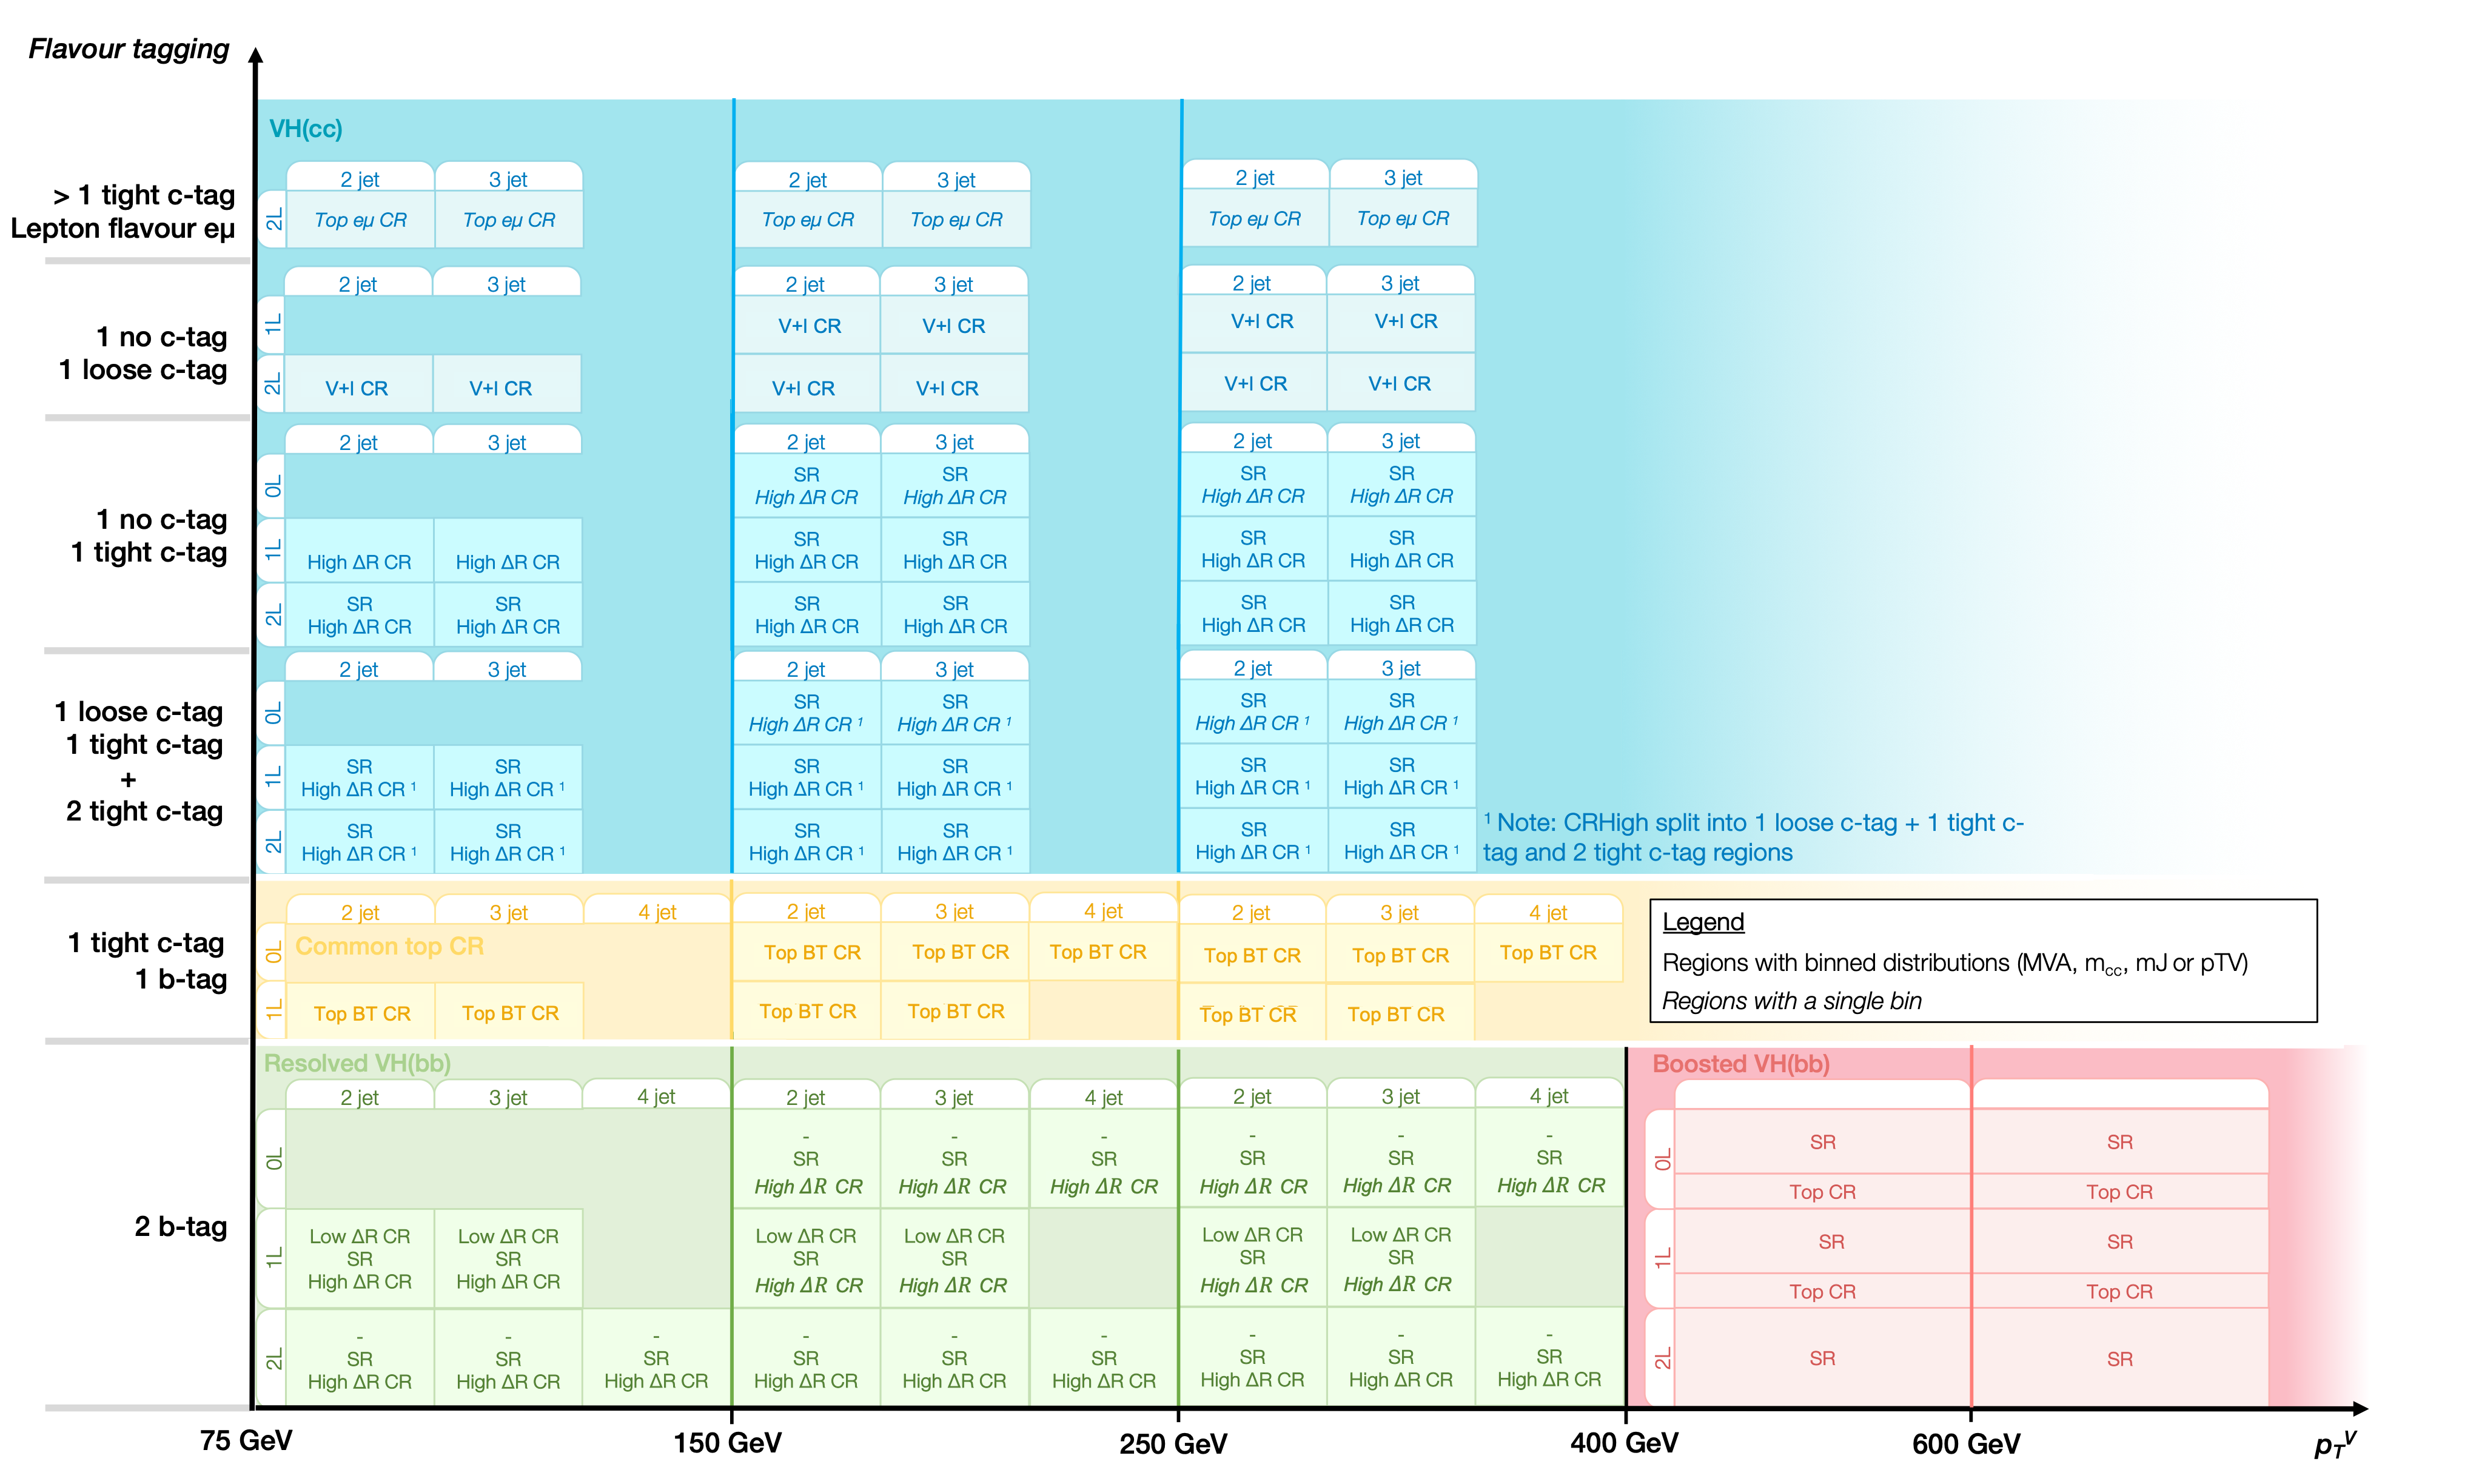
\includegraphics[width=\textwidth]{Images/VH/Cat/VH_analysis_catCorr.png}
    \caption{The combined \vhbc\ analysis regions, showing the Signal Regions (SRs), High and Low $\Delta R$ control regions (CRHighs and CRLows), the top $BT$ CRs, the top $e\mu$ CRs, the $V+l$ $LN$-tagged CRs, and the boosted top CRs. \vhc\ is in blue, the shared top $BT$ CRs in the resolved regime in yellow, and \vhb\ in green and red for the resolved and boosted regimes respectively. Regions used in the fit as single-bin distributions to derive an absolute normalisation are indicated in italics.} 
    \label{fig:ana-strat-det}
\end{sidewaysfigure} 

\clearpage

\subsection{Event Categorisation}\label{sec-eventCat}
Selected events are finely categorised following a successive decomposition into regions of defined flavour tag, vector boson $V$ transverse momentum $p_T^V$, and number of jets \nj. The full categorisation gives rise to signal and control regions that enter the statistical analysis defined in the fit framework of Section~\ref{sec-fitFramework}. The control regions are defined to constrain the modelling of specific backgrounds. The definition of the regions depends on the analysis regime and the targeted Higgs decay mode, with Figure~\ref{fig:ana-strat-det} providing a condensed global overview.

\subsubsection{Resolved Regime Categorisation}
In the resolved regime, the number of central and forward jets in an event defines different \nj\ categories, separated to maximise the signal sensitivity. A $p_T > 30$ GeV cut is applied to non-Higgs candidate jets when determining the jet multiplicity for the categorisation. This requirement limits the signal migration across \gls{stxs} bins in \vhb, with almost no impact to the \vhc\ sensitivity. All distributions of the resolved regime regions with processes normalised to their postfit expectations from the fit described in Section~\ref{sec-fitFramework} are presented in Appendix \ref{appsec-vh-analRegPosfit}. The plots presented in this section show the prefit blinded distributions in the different regions, and simulated processes are therefore not normalised to data. The distributions displayed correspond to those chosen for the fit, as detailed in Section~\ref{sec-vh-disc}. The precise definitions of the analysis regions are reviewed in this section.

\paragraph{Resolved \boldvhb\ SRs:} require exactly 2 $b$-tagged jets ($BB$), with no extra $B$- nor any $T$-tags, and events are separated into different categories based on \nj. All lepton channels have a 2-jet and a 3-jet categories. The 0L channel has an additional 4-jet category, and the 2L an extra 4 or more jets (4p or $\geq$4) category. They are included to improve the \gls{stxs} measurements sensitivity in bins with at least one additional jet. All regions are further split into different bins of $p_T^V$ as [75, 150] GeV\footnote{This region is not included in 0L due to the $E_T^{\textrm{miss}}$ trigger threshold.}, [150, 250] GeV, and [250, 400] GeV. Some selected \vhb\ signal regions in the analysis are presented in Figure~\ref{fig:plots_VHbb_ex_SR}, showing the distributions of the \glspl{bdt} introduced in Section \ref{sec-vh-disc}. 

\begin{figure}[h!]
  \centering
  \begin{subfigure}[b]{0.32\textwidth}
      \centering
      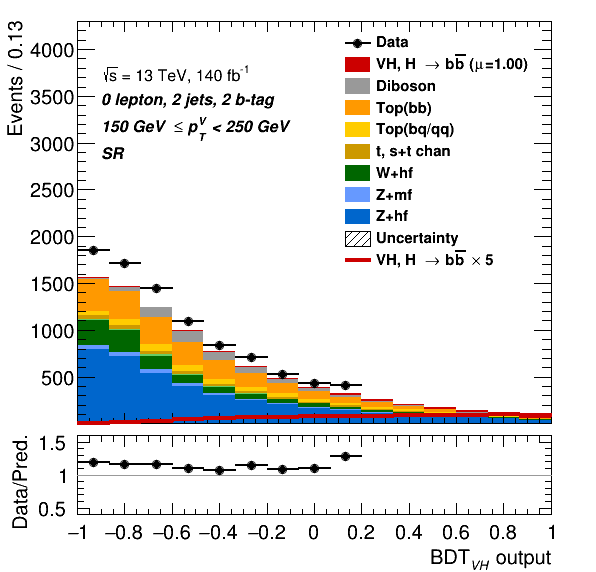
\includegraphics[width=\textwidth]{Images/VH/Own_fit/prefit_VHbb/Region_distmva_BMax250_BMin150_DSR_J2_TTypebb_T2_L0_Y6051_Prefit.png}
      \caption{0-lepton.}
      \label{fig:plots_VHbb_ex_OL_SR}
  \end{subfigure}
  \begin{subfigure}[b]{0.32\textwidth}
      \centering
      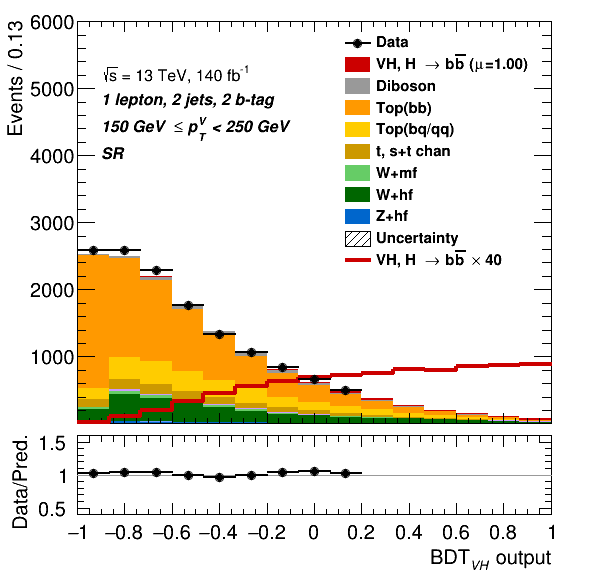
\includegraphics[width=\textwidth]{Images/VH/Own_fit/prefit_VHbb/Region_distmva_BMax250_BMin150_DSR_J2_TTypebb_T2_L1_Y6051_Prefit.png}
      \caption{1-lepton}
      \label{fig:plots_VHbb_ex_1L_SR}
  \end{subfigure}
  \begin{subfigure}[b]{0.32\textwidth}
    \centering
    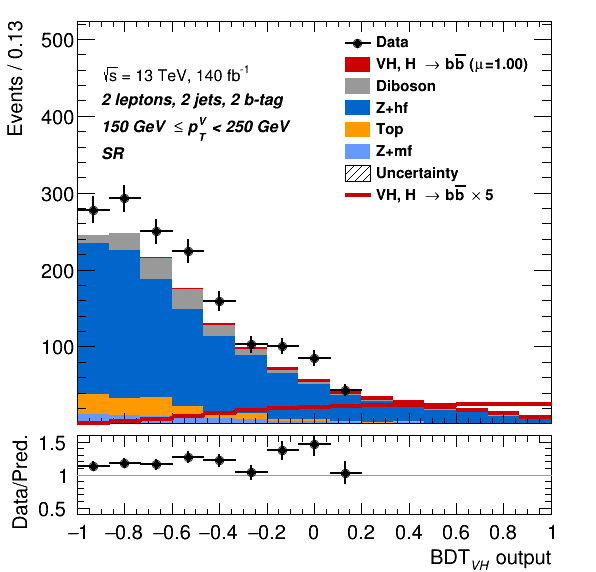
\includegraphics[width=\textwidth]{Images/VH/Own_fit/prefit_VHbb/Region_distmva_BMax250_BMin150_DSR_J2_TTypebb_T2_L2_Y6051_Prefit.png}
    \caption{2-lepton.}
    \label{fig:plots_VHbb_ex_2L_SR}
\end{subfigure}
  \caption{\gls{bdt} distributions for the $BB$-tagged 2-jet signal regions with 150 GeV < \ptv\ < 250 GeV for different lepton channels.}
  \label{fig:plots_VHbb_ex_SR}
\end{figure} 

\paragraph{Resolved \boldvhc\ SRs:} adopt a similar event categorisation to the resolved \vhb, with at least one candidate jet being tight c-tagged $T$. The categorisation of the signal region is then split based on the remaining candidate tag into a 2 $c$-tags region and a 1 $c$-tag region. The former requires an extra tight ($TT$) or loose $c$-tag ($LT$)\footnote{The 2 $c$-tagged labelled $LT+TT$ is summarised as $XT$ in the plots.}, the latter an untagged jet $N$ ($NT$). The $p_T^V$ bins are similar to \vhb, except for the highest $p_T^V$ one that is relaxed to $\geq 250$ GeV given the limited impact of the overlap with the boosted \vhb. Adding the \ptv\ region above 400 GeV was found to increase the total \vhc\ sensitivity by 10\%. The jet multiplicity, \nj, defines a 2 and a 3 jets categories, with the latter extended to 3 or more jets (3p or $\geq$3) in 2L due to a reduced \ttb\ background. A selection of 2 $c$-tagged signal regions is presented in Figure~\ref{fig:plots_VHcc_ex_SR_2C}, with Figure~\ref{fig:plots_VHcc_ex_SR_1C} presenting some 1 $c$-tagged signal regions. The 1 $c$-tag \glspl{sr} in the 75 GeV $<$ \ptv\ $<$ 150 GeV range are not included in the fit because of their significant background contamination.

\begin{figure}[h!]
  \centering
  \begin{subfigure}[b]{0.32\textwidth}
      \centering
      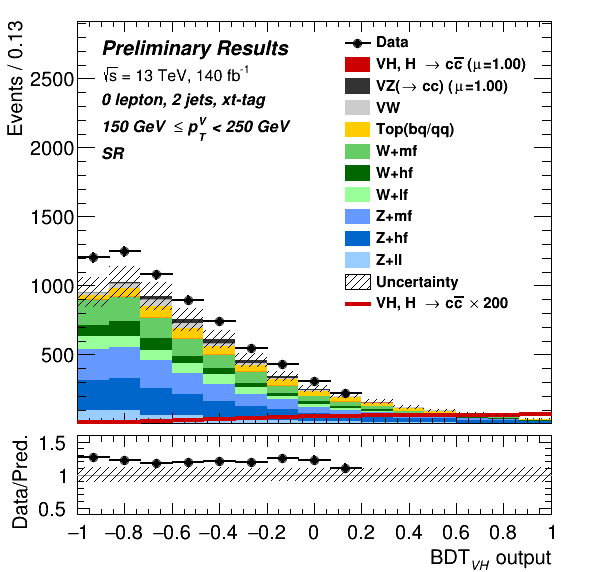
\includegraphics[width=\textwidth]{Images/VH/Own_fit/prefit_VHcc/Region_distmva_BMax250_BMin150_DSR_J2_TTypext_T2_L0_Y6051_Prefit.png}
      \caption{0-lepton, 2-jet.}
      \label{fig:plots_VHcc_ex_OL_SR_2C}
  \end{subfigure}
  \begin{subfigure}[b]{0.32\textwidth}
      \centering
      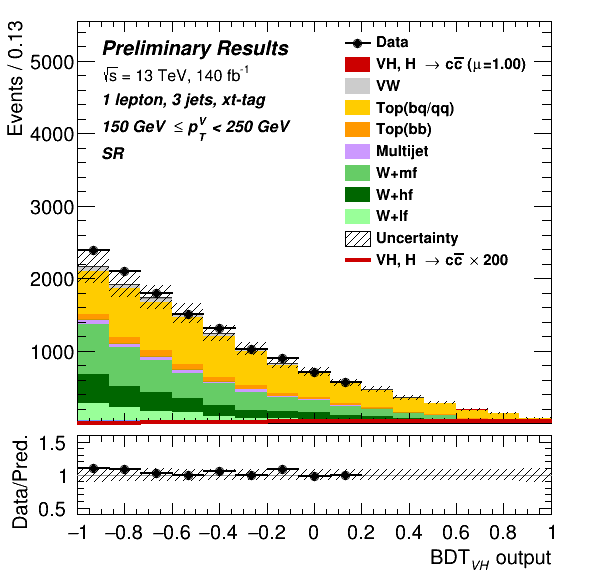
\includegraphics[width=\textwidth]{Images/VH/Own_fit/prefit_VHcc/Region_distmva_BMax250_BMin150_DSR_J3_TTypext_T2_L1_Y6051_Prefit.png}
      \caption{1-lepton, 3-jet.}
      \label{fig:plots_VHcc_ex_1L_SR_2C}
  \end{subfigure}
  \begin{subfigure}[b]{0.32\textwidth}
    \centering
    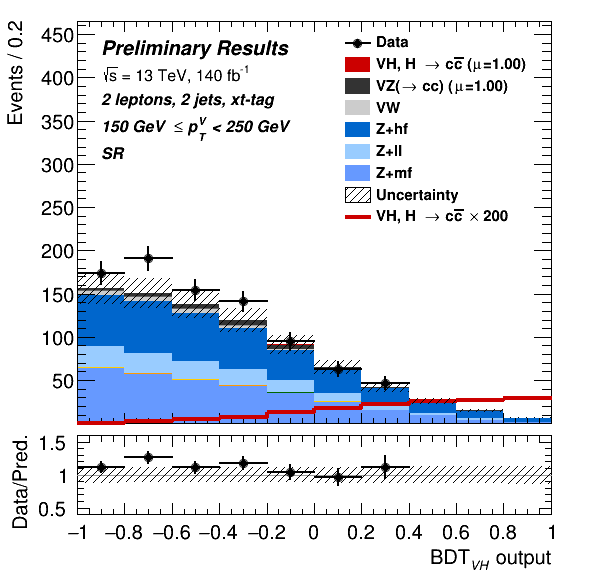
\includegraphics[width=\textwidth]{Images/VH/Own_fit/prefit_VHcc/Region_distmva_BMax250_BMin150_DSR_J2_TTypext_T2_L2_Y6051_Prefit.png}
    \caption{2-lepton, 2-jet.}
    \label{fig:plots_VHcc_ex_2L_SR_2C}
\end{subfigure}
  \caption{\gls{bdt} distributions for 2 $c$-tagged ($TT$ + $LT$) signal regions with 150 GeV < \ptv\ < 250 GeV, for different lepton channels and jet multiplicities.}
  \label{fig:plots_VHcc_ex_SR_2C}
\end{figure} 


\begin{figure}[h!]
  \centering
  \begin{subfigure}[b]{0.32\textwidth}
      \centering
      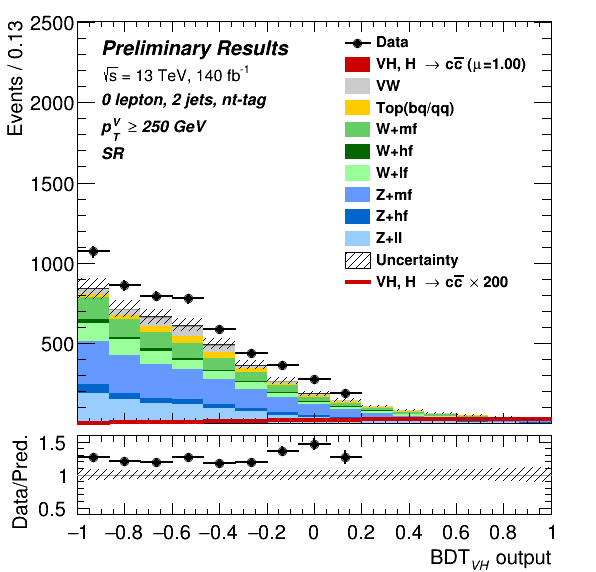
\includegraphics[width=\textwidth]{Images/VH/Own_fit/prefit_VHcc/Region_distmva_BMin250_DSR_J2_TTypent_T1_L0_Y6051_Prefit.png}
      \caption{0-lepton, 2-jet.}
      \label{fig:plots_VHcc_ex_OL_SR_1C}
  \end{subfigure}
  \begin{subfigure}[b]{0.32\textwidth}
      \centering
      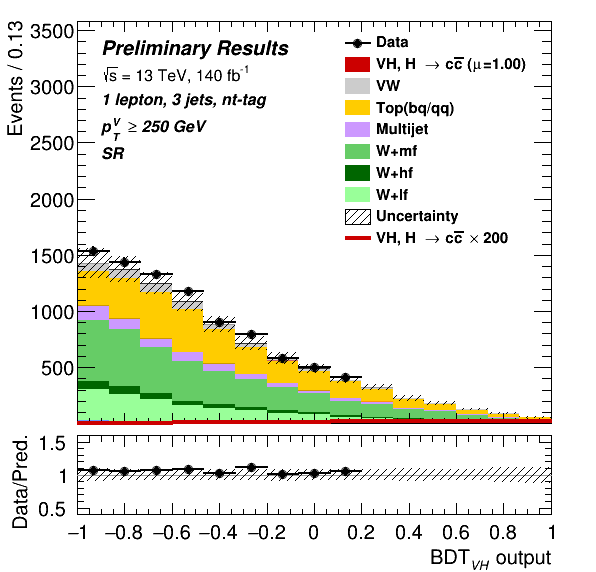
\includegraphics[width=\textwidth]{Images/VH/Own_fit/prefit_VHcc/Region_distmva_BMin250_DSR_J3_TTypent_T1_L1_Y6051_Prefit.png}
      \caption{1-lepton, 3-jet.}
      \label{fig:plots_VHcc_ex_1L_SR_1C}
  \end{subfigure}
  \begin{subfigure}[b]{0.32\textwidth}
    \centering
    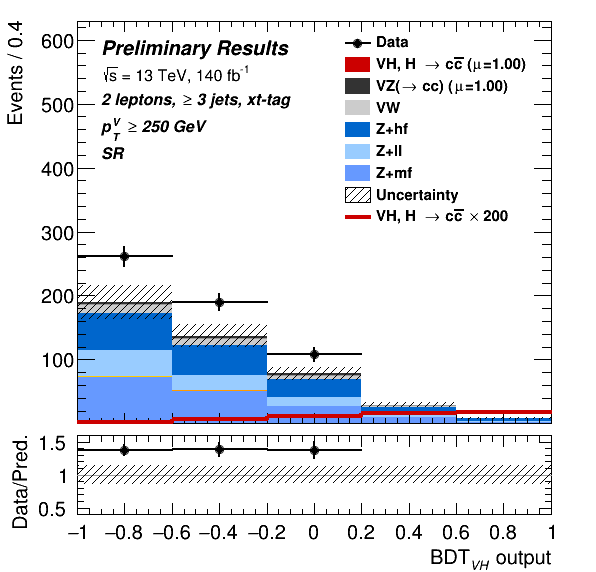
\includegraphics[width=\textwidth]{Images/VH/Own_fit/prefit_VHcc/Region_distmva_BMin250_DSR_J3_TTypext_incJet1_T2_L2_Y6051_Prefit.png}
    \caption{2-lepton, $\geq$ 3 (3p) jets.}
    \label{fig:plots_VHcc_ex_2L_SR_1C}
\end{subfigure}
  \caption{\gls{bdt} distributions for 1 $c$-tagged signal regions with 250 < \ptv.}
  \label{fig:plots_VHcc_ex_SR_1C}
\end{figure} 

\paragraph{High $\boldsymbol{\Delta R}$ Control Regions:} are designed to constrain the normalisation and shape of the $V+$jets and the \ttb\ background when the 2 candidate jets are the $b$-quarks. They are defined by a further split from the \glspl{sr} based on the angular separation $\Delta R(j_1, j_2)$, denoted as $\Delta R$, between the Higgs candidate jets. This split is governed by a $p_T^V$-dependent cut on the $\Delta R$ that is derived to keep 95\% (85\%) of the signal yield in the 2-jet (3 or more jets) \glspl{sr}. The cuts are defined in Table \ref{tbl:CRhigh_definition} and illustrated in Figure~\ref{fig:drccptvCutsVHcc}, with their derivation detailed in Appendix~\ref{ap-sec-vh-deltaR}. Events with a $\Delta R$ below the selection line enter the signal region, while those above go in a \highdr\ \gls{cr}, also called \textit{CRHigh}. To avoid some mismodelling effect at high $\Delta R$ and to keep the \highdr\ \gls{cr} kinematically close to the \gls{sr}, an uppercut of $\Delta R \leq \pi$ is applied to all events. This effectively removes $\sim 40$\% of events in the \highdr\ \gls{cr}, with a negligible impact on the signal region. For \vhc, CRHighs are defined separately for 1 and 2 $c$-tagged events. The $TT$- and $LT$-tagged events are also separated to constrain the \vhf\ and \vmf\ backgrounds. In \vhb, the CRHighs are used to extract the normalisation of the backgrounds while in \vhc\ the shapes of the $m_{c\bar{c}}$ and \ptv\ spectrum are also used, as detailed in Section~\ref{sec-vh-disc}. Several \highdr\ \glspl{cr} are shown in Figure~\ref{fig:plots_VHcc_ex_CRH}. %\footnote{$\Delta R(j_1, j_2) = \sqrt{(\eta_{j_1} - \eta_{j_2})^2 + (\phi_{j_1} - \phi_{j_2})^2 }$.}
\begin{table}[htbp]
  \centering
  \begin{tabular}{c|c|c}
    \hline
    \hline
    Category & \highdr & \lowdr \\ \hline
    $2$-jet & $ \Delta R > 0.787 + e^{1.387 - 0.0070 \times p_{T}^{V} } $      &  $ \Delta R < 0.410 + e^{ 0.818 - 0.0106  \times p_{T}^{V} } $        \\
    $3$-jet & $ \Delta R > 0.684 + e^{1.204 - 0.0060 \times p_{T}^{V} } $      &  $ \Delta R < 0.430 + e^{ 0.399 - 0.0093  \times p_{T}^{V} } $        \\
    $4$-jet & $ \Delta R > 0.863 + e^{0.984 - 0.0041 \times p_{T}^{V} } $ &  $ \Delta R < 0.411 + e^{ 1.204 - 0.0060  \times p_{T}^{V} } $        \\
    $\geq$5-jet & $ \Delta R > 1.667 + e^{0.519 - 0.0050 \times p_{T}^{V} } $ &  $ \Delta R < 0.501 + e^{ 1.192 - 0.0075  \times p_{T}^{V} } $      \\
    \hline
    \hline
  \end{tabular}
  \caption{Cuts defining the \highdr\ (centre - CRHigh) and \lowdr\ (right - CRLow) control regions. The inequalities are set to enter the control regions, with \ptv\ expressed in GeV.}
  \label{tbl:CRhigh_definition}
\end{table}
  
\paragraph{Low $\Delta R$ Control Regions:} \lowdr\ \glspl{cr} (\textit{CRLows}) are defined in the 1-lepton channel of \vhb\ to better constrain the \whf\ background. They are based on \ptv-dependant cuts defined similarly to the \highdr\ ones, separating 10\% of the diboson events from the signal regions, as displayed in the bottom parts of the plots in Figure~\ref{fig:drccptvCutsVHcc}. The selection criteria are defined in the right of Table \ref{tbl:CRhigh_definition}, where events with a $\Delta R$ above the cutting line enter the signal region while those below belong to the CRLow. In \vhc\ and the 0L and 2L \vhb, the CRLow is not separated from the signal region as it has little impact on the sensitivity of the fit. A CRLow regions is presented in Figure~\ref{fig:plots_VHb_ex_1L_CRL}.

\begin{figure}[h!]
  %\hspace{-2.0cm}
  \center
  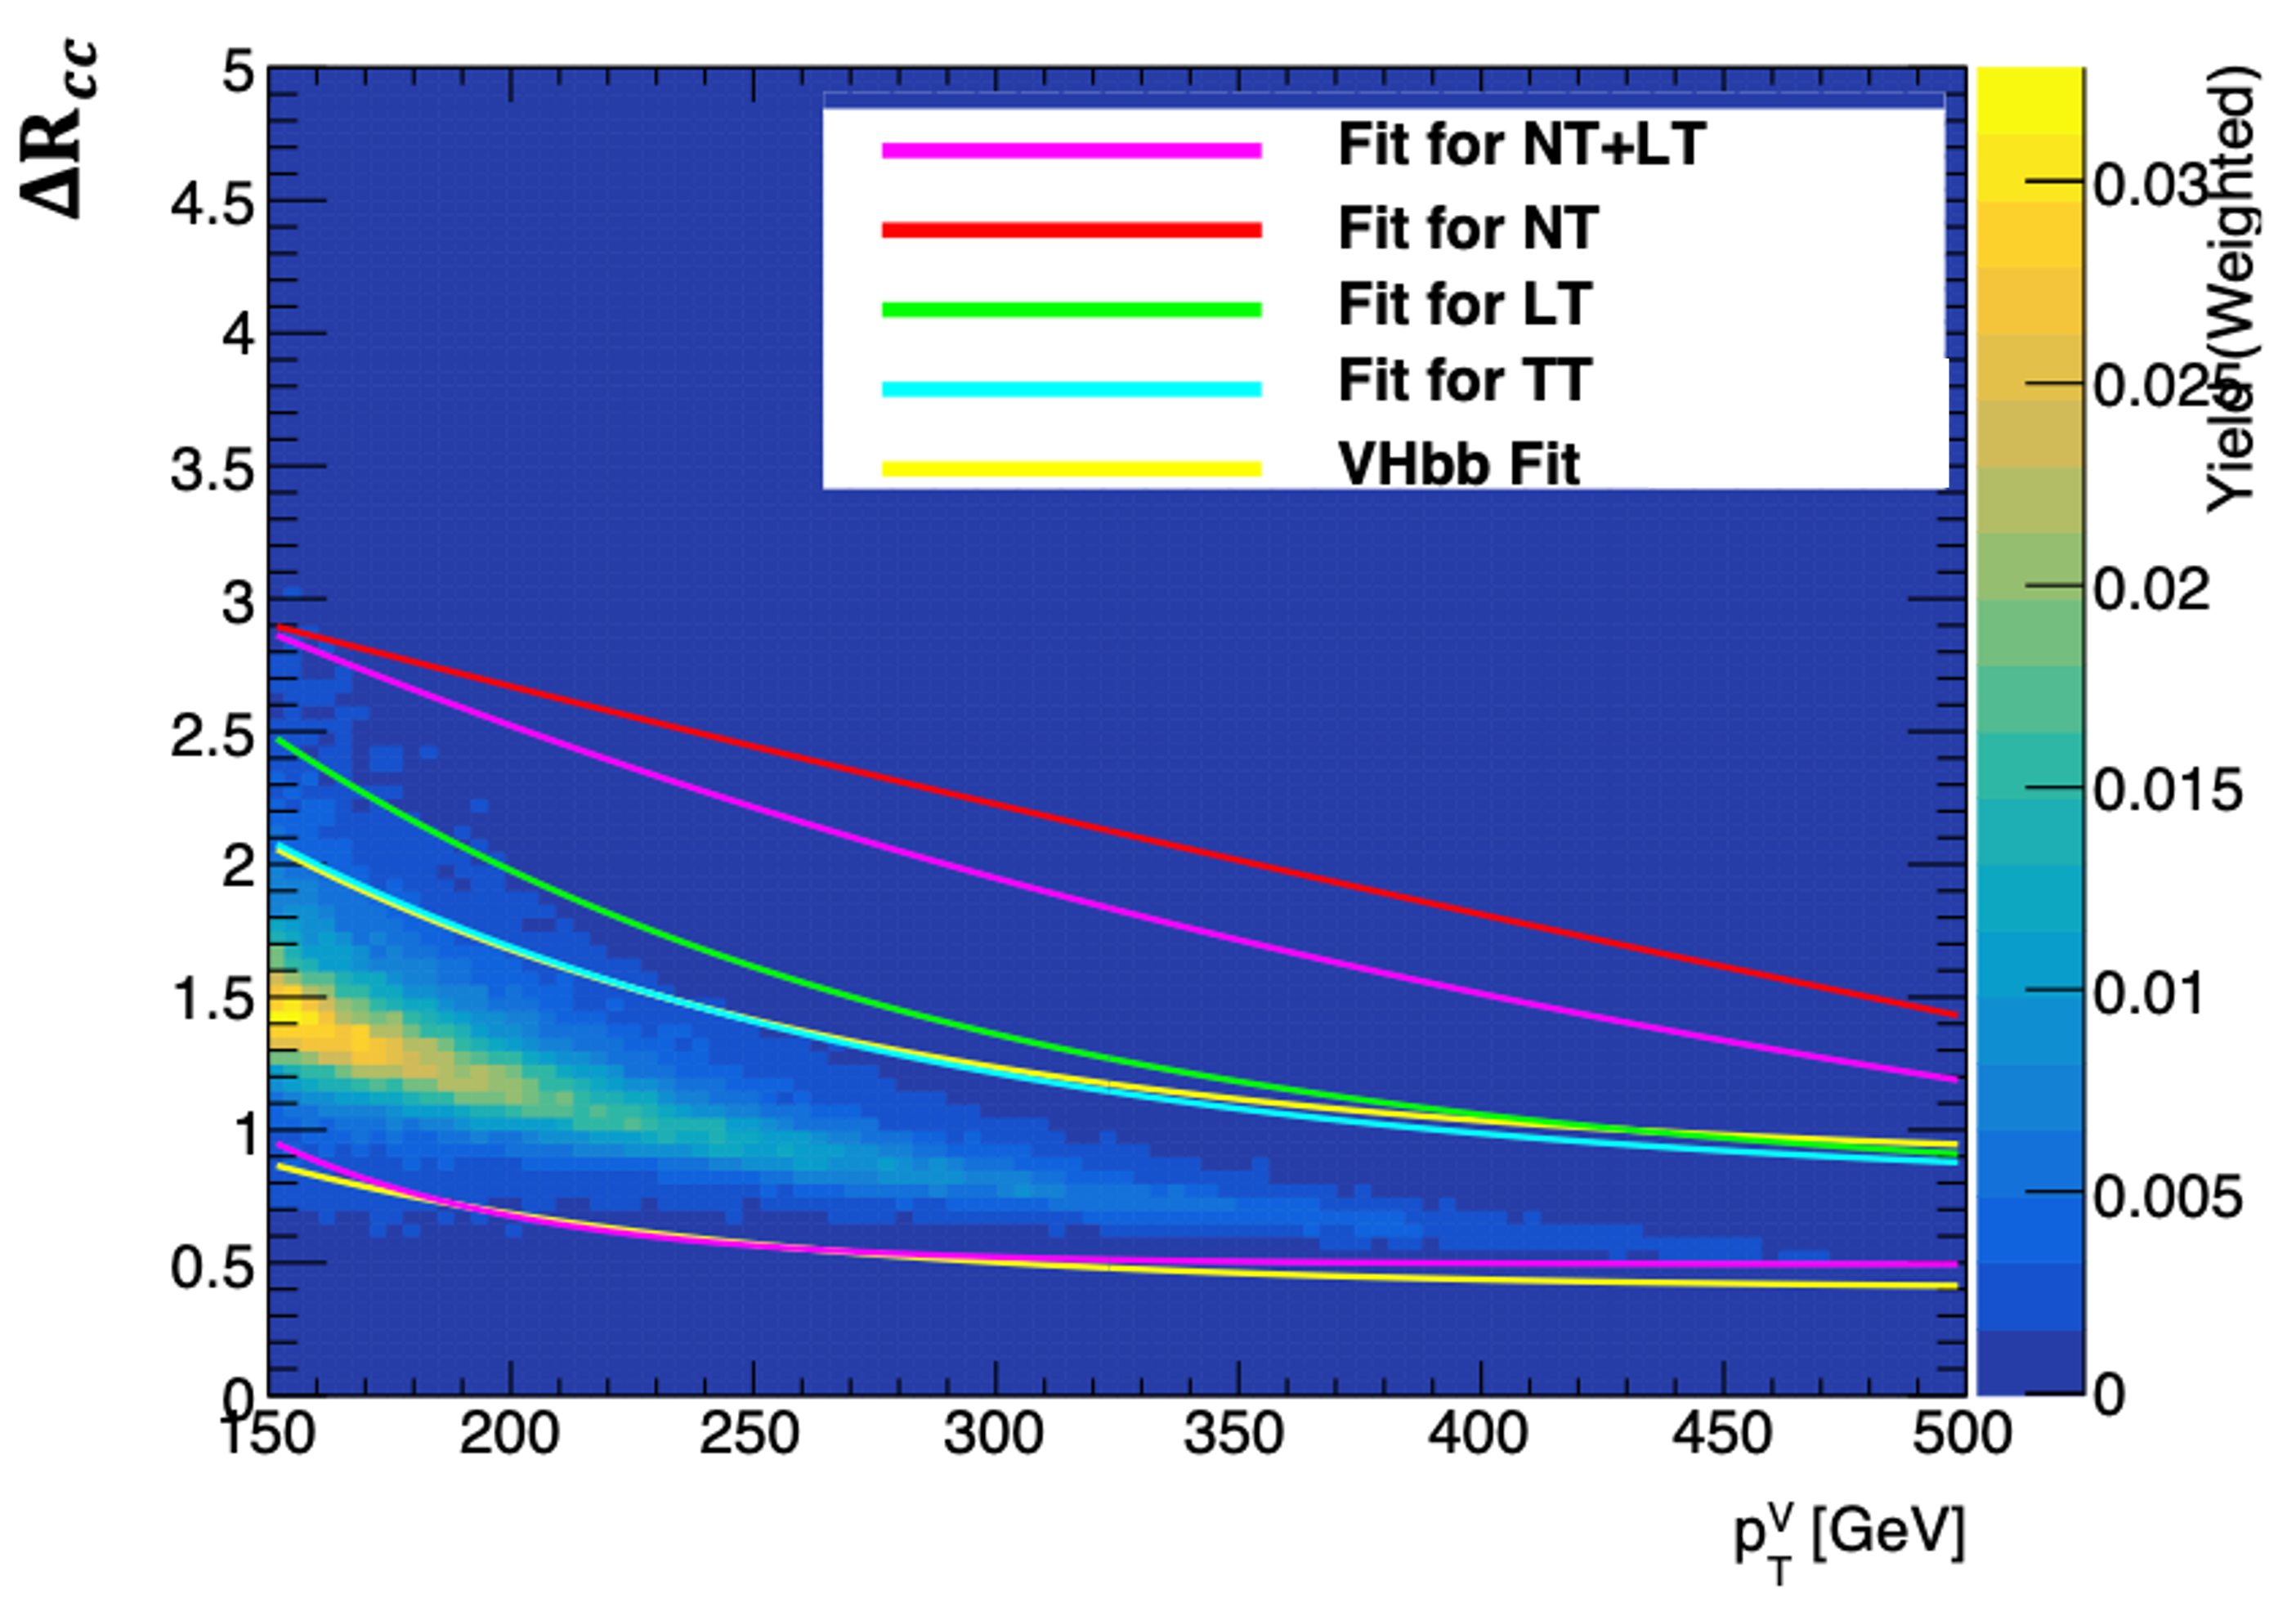
\includegraphics[width=0.48\textwidth]{Images/VH/dRccpTV/sr1.png}
  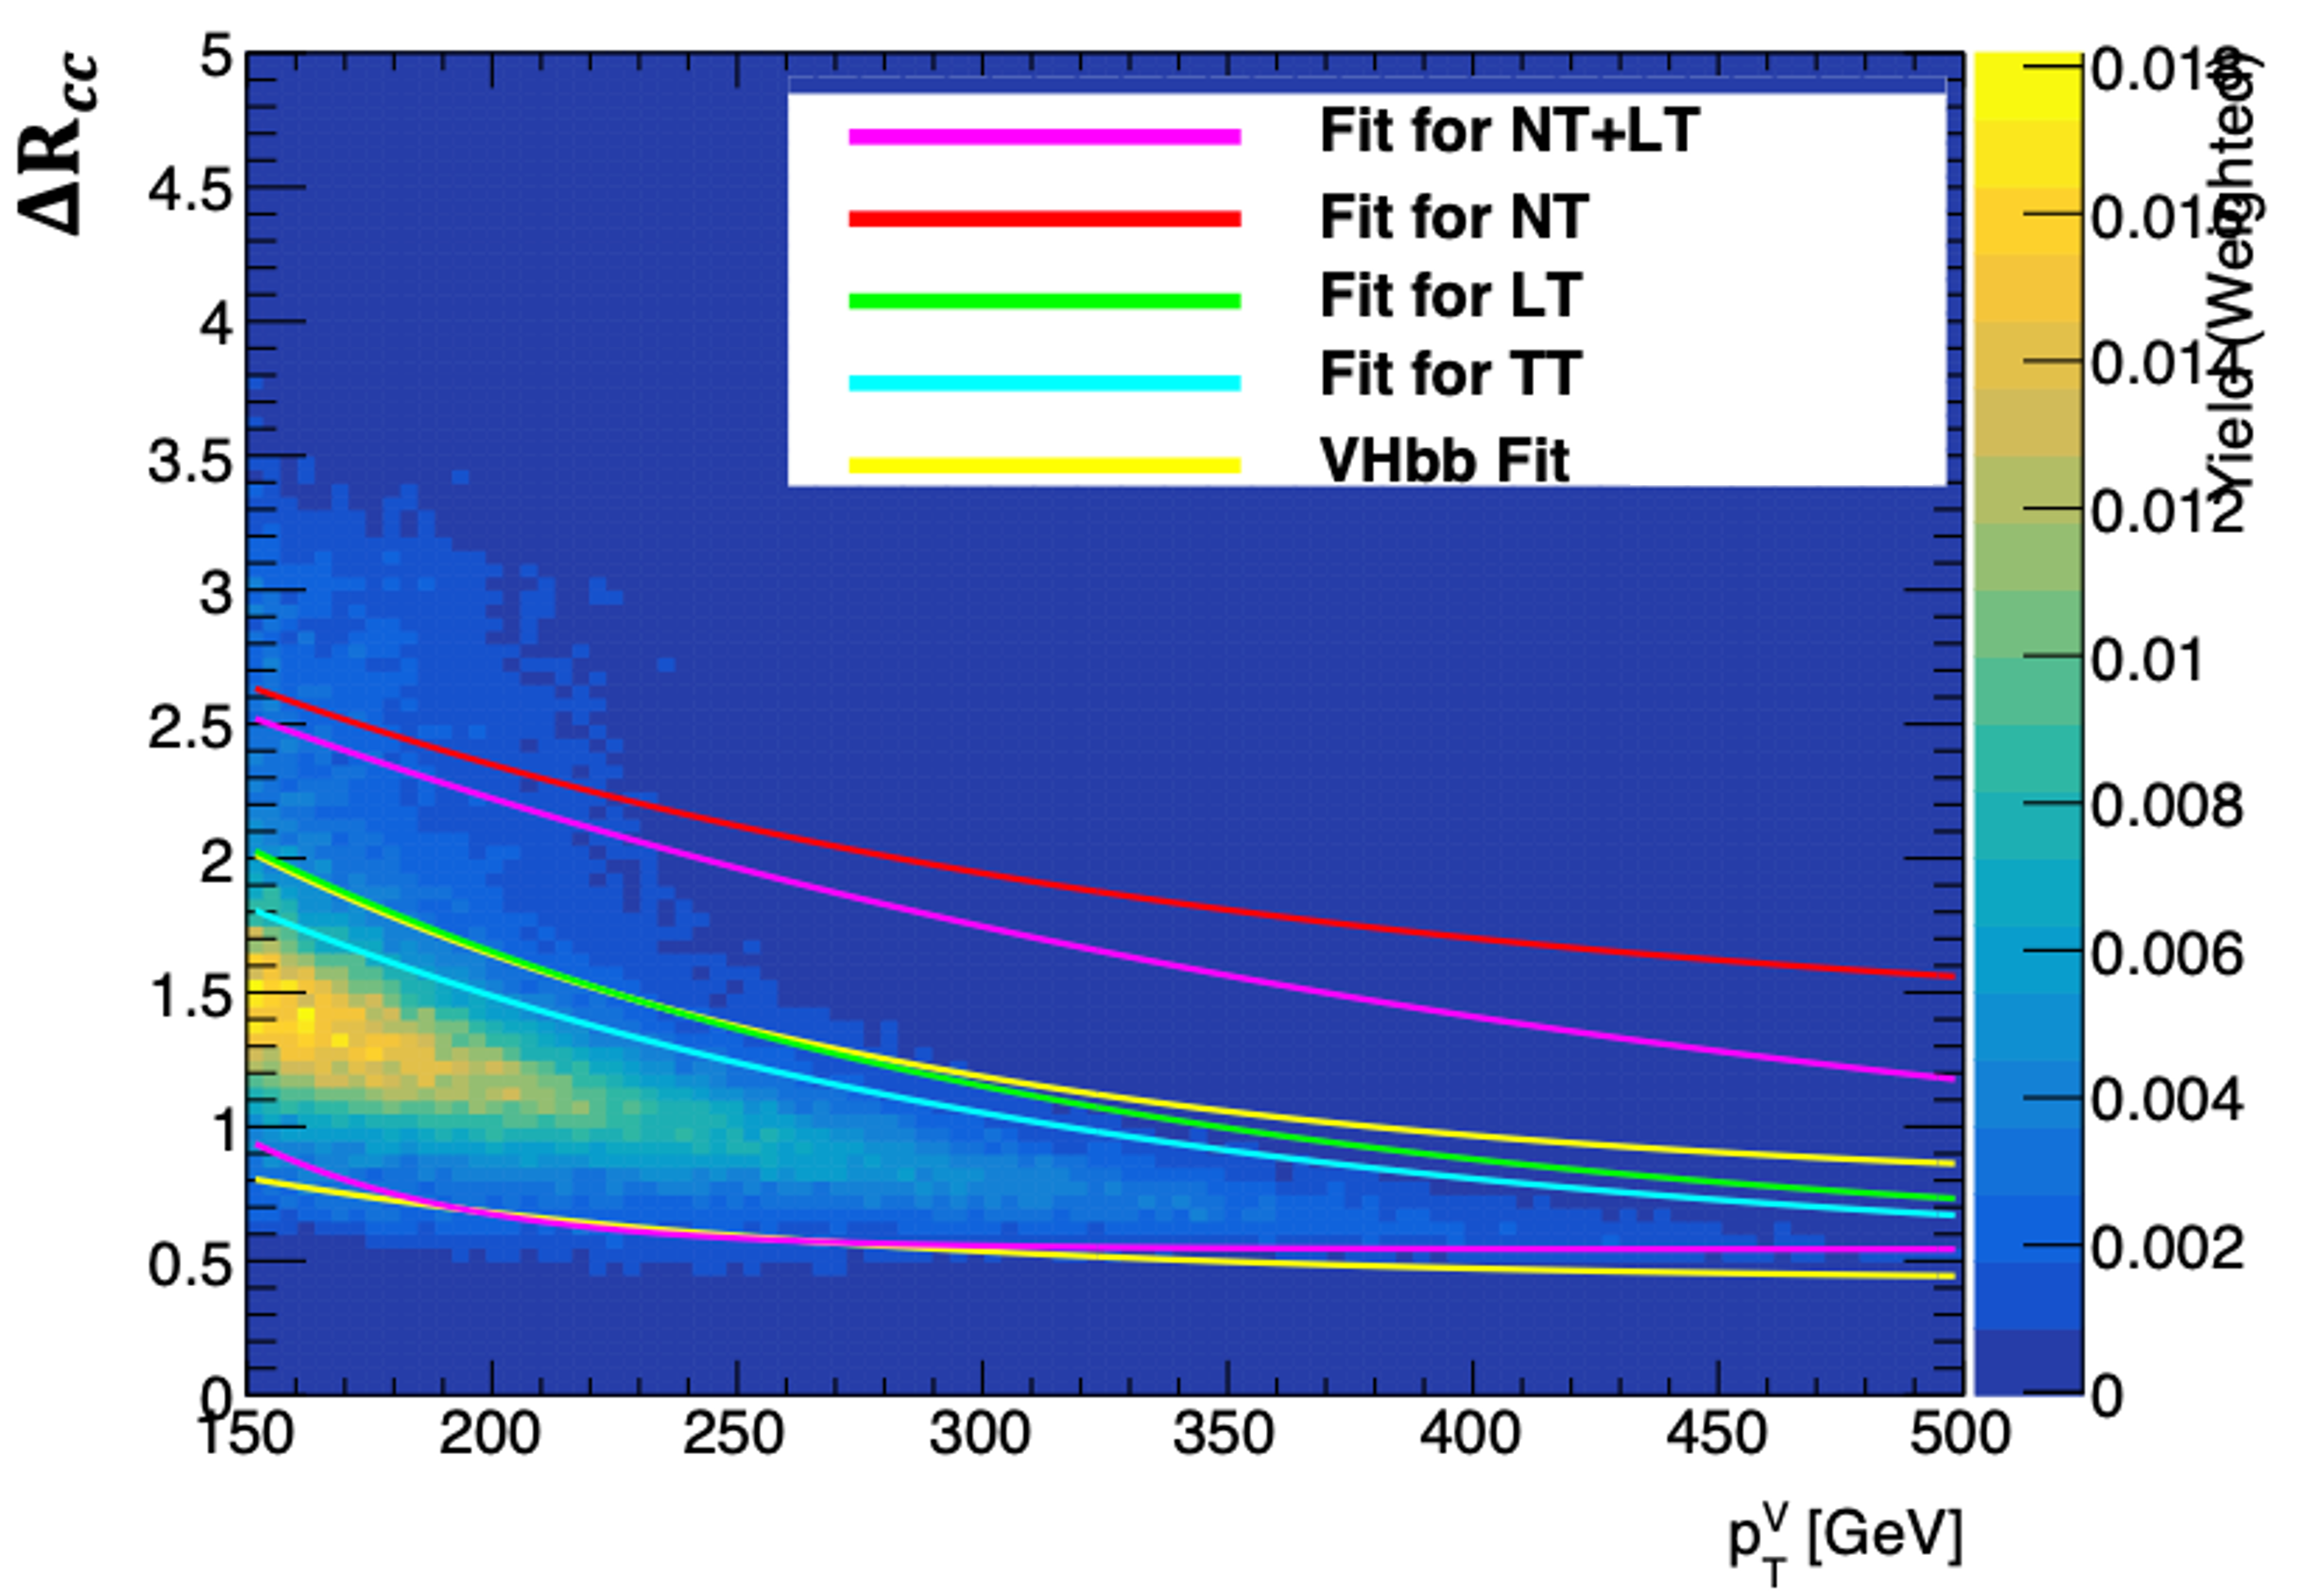
\includegraphics[width=0.48\textwidth]{Images/VH/dRccpTV/sr2.png}
  \caption{The $p_T^V$-$\Delta R_{c\bar{c}}$ 2D signal yield map of the 1L \vhc, for the 2-jet (left) and 3-jet (right) regions. The lines are the results of fitting the high and low $\Delta R_{c\bar{c}}(p_T^V)$ cuts for various signal tags, with the yellow curve showing the $\Delta R_{b\bar{b}}$ cut from \vhb that is used in the analysis. The CRHigh is above the top yellow line and the SR below. A \lowdr\ CR can be defined by the bottom lines, splitting this region from the SR for the \vhb\ only.} 
  \label{fig:drccptvCutsVHcc}
\end{figure}

\begin{figure}[h!]
  \centering
  \begin{subfigure}[b]{0.32\textwidth}
      \centering
      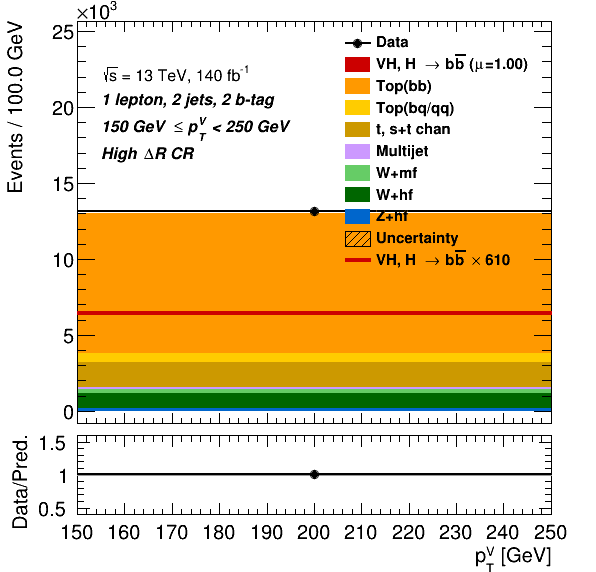
\includegraphics[width=\textwidth]{Images/VH/Own_fit/prefit_VHbb/Region_distpTV_BMax250_BMin150_DCRHigh_J2_TTypebb_T2_L1_Y6051_Prefit.png}
      \caption{1-lepton $BB$, \ptv\ distribution.}
      \label{fig:plots_VHcc_ex_OL_CRH}
  \end{subfigure}
  \begin{subfigure}[b]{0.32\textwidth}
      \centering
      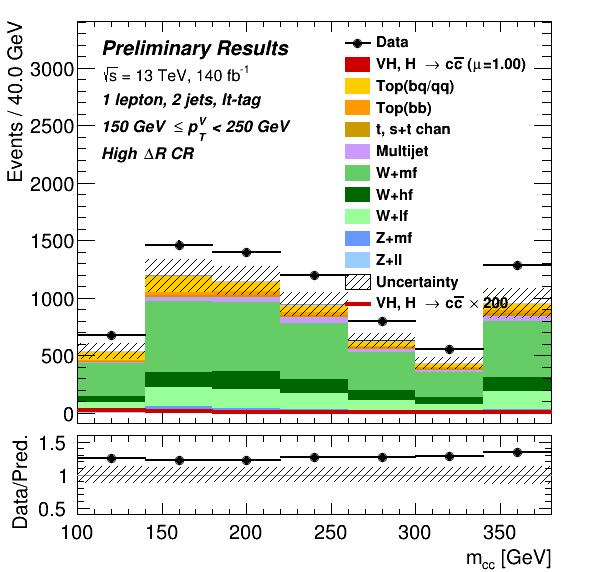
\includegraphics[width=\textwidth]{Images/VH/Own_fit/prefit_VHcc/Region_distmBB_BMax250_BMin150_DCRHigh_J2_TTypelt_T2_L1_Y6051_Prefit.png}
      \caption{1-lepton $LT$, $m_{c\bar{c}}$ distribution.}
      \label{fig:plots_VHcc_ex_1L_CRH}
  \end{subfigure}
  \begin{subfigure}[b]{0.32\textwidth}
    \centering
    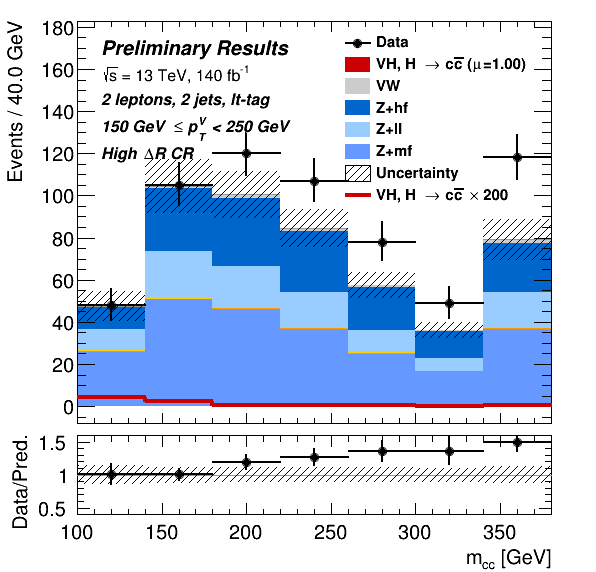
\includegraphics[width=\textwidth]{Images/VH/Own_fit/prefit_VHcc/Region_distmBB_BMax250_BMin150_DCRHigh_J2_TTypelt_T2_L2_Y6051_Prefit.png}
    \caption{2-lepton $LT$, $m_{c\bar{c}}$ distribution.}
    \label{fig:plots_VHcc_ex_2L_CRH}
\end{subfigure}
  \caption{Some \highdr\ \glspl{cr} (CRHigh) with 2 jets and 150 GeV < \ptv\ < 250 GeV.}
  \label{fig:plots_VHcc_ex_CRH}
\end{figure} 

\paragraph{Top Control Regions in 0L and 1L:} are defined to constrain the top background top($bc$) and top($bl$) components\footnote{The component in parenthesis refers to the flavour of the Higgs candidate jets.}, where \textit{top} is the combination of the \ttb\ and single-top $Wt$ processes. The so-called \textit{top $BT$ CRs} are shared by the resolved \vhb\ and \vhc, with the same \ptv\ and jet multiplicity categorisation as in the \glspl{sr}.  They are defined for 0L and 1L by requiring events to have at least one $B$-tag and at least one tight $c$-tag $T$, making them orthogonal to the signal regions. The Higgs candidate is reconstructed from the leading $B$-tagged and $T$- tagged jets, for kinematic similarity to the \glspl{sr}. The top($bb$) component, a major background in \vhb, is controlled from the previously defined CRHighs, thanks to the large $\Delta R$ between the produced $b$ jets in \ttb\ events, as shown in Figure~\ref{fig:plots_VHcc_ex_OL_CRH}. Two top $BT$ control regions are presented on the left of Figure~\ref{fig:plots_VHcc_ex_TopCR}.

\begin{figure}[h!]
  \centering
  \begin{subfigure}[b]{0.32\textwidth}
      \centering
      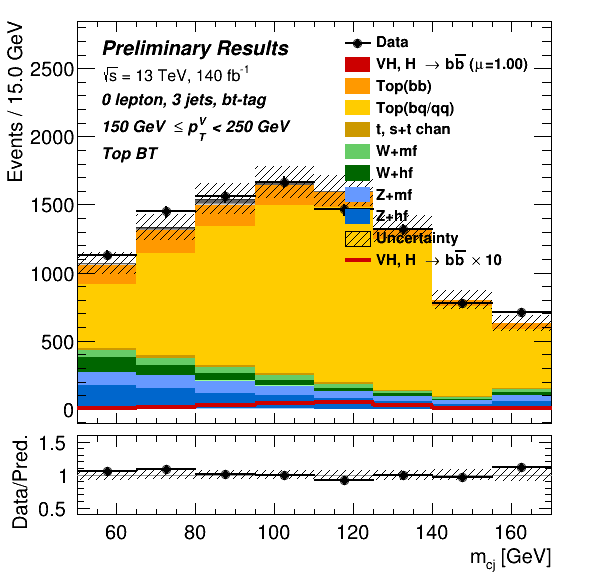
\includegraphics[width=\textwidth]{Images/VH/Own_fit/prefit_VHcc/Region_distmBB_BMax250_BMin150_DtopCRBC_J3_TTypebt_T1_L0_Y6051_Prefit.png}
      \caption{0-lepton, $BT$, 3-jet.}
      \label{fig:plots_VHcc_ex_OL_TopCR}
  \end{subfigure}
  \begin{subfigure}[b]{0.32\textwidth}
      \centering
      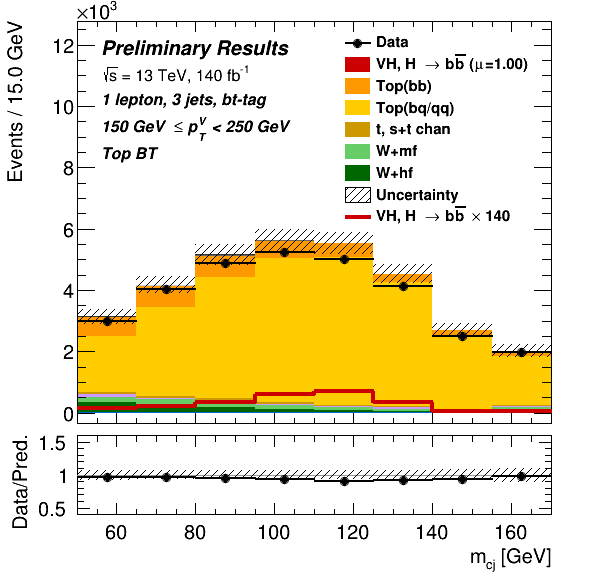
\includegraphics[width=\textwidth]{Images/VH/Own_fit/prefit_VHcc/Region_distmBB_BMax250_BMin150_DtopCRBC_J3_TTypebt_T1_L1_Y6051_Prefit.png}
      \caption{1-lepton, $BT$, 3-jet.}
      \label{fig:plots_VHcc_ex_1L_TopCR}
  \end{subfigure}
  \begin{subfigure}[b]{0.32\textwidth}
    \centering
    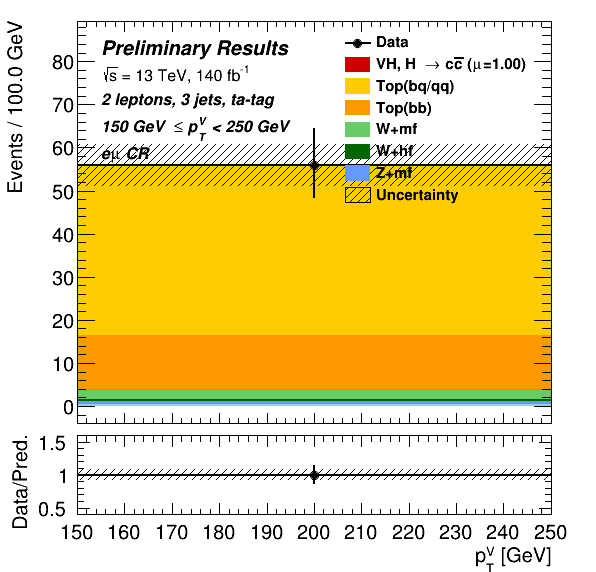
\includegraphics[width=\textwidth]{Images/VH/Own_fit/prefit_VHcc/Region_distpTV_BMax250_BMin150_Dtopemucr_J3_TTypeta_T2_L2_Y6051_Prefit.png}
    \caption{2-lepton, $e\mu$, $\geq$ 1 $T$-tag.}
    \label{fig:plots_VHcc_ex_2L_TopCR}
\end{subfigure}
  \caption{Top $BT$-tagged (left and centre - $m_{cj}$ distribution) and $e\mu$ (right - \ptv\ distribution) CRs, with 3 jets and 150 GeV < \ptv\ < 250 GeV.}
  \label{fig:plots_VHcc_ex_TopCR}
\end{figure} 

\paragraph{Top Control Regions in 2L:} the top background in 2L is mostly made of di-leptonic \ttb\ decays, with both subsequent $W$ decaying leptonically. High purity top \glspl{cr} are derived for the 2-lepton channels by requiring leptons of different flavours ($e\mu$ / $\mu e$) instead of the same flavour ($ee$ / $\mu\mu$). This mix of flavours is possible as the leptons are produced in distinct $W$ boson decays. These so-called \textit{top} $e\mu$ \textit{CRs} are used to derive a \ttb\ background template in a data-driven way for the 2-lepton \glspl{sr} in \vhb. For \vhc, the \ttb\ is a less significant background in 2L due to the flavour tagging requirements, and the top $e\mu$ \glspl{cr} contribute to the fit as a single-bin \glspl{cr} defined per \ptv\ and jet multiplicity, with at least one $T$-tag jet. An example of these \glspl{cr} is presented in Figure~\ref{fig:plots_VHcc_ex_2L_TopCR}.

\begin{figure}[h!]
  \centering
  \begin{subfigure}[b]{0.32\textwidth}
      \centering
      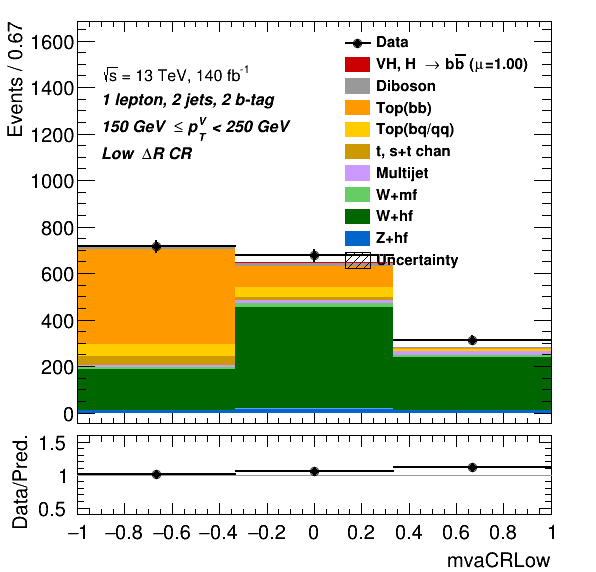
\includegraphics[width=\textwidth]{Images/VH/Own_fit/prefit_VHbb/Region_distmvaCRLow_BMax250_BMin150_DCRLow_J2_TTypebb_T2_L1_Y6051_Prefit.png}
      \caption{1-lepton \lowdr\ CR, $BB$.}
      \label{fig:plots_VHb_ex_1L_CRL}
  \end{subfigure}
  \begin{subfigure}[b]{0.32\textwidth}
      \centering
      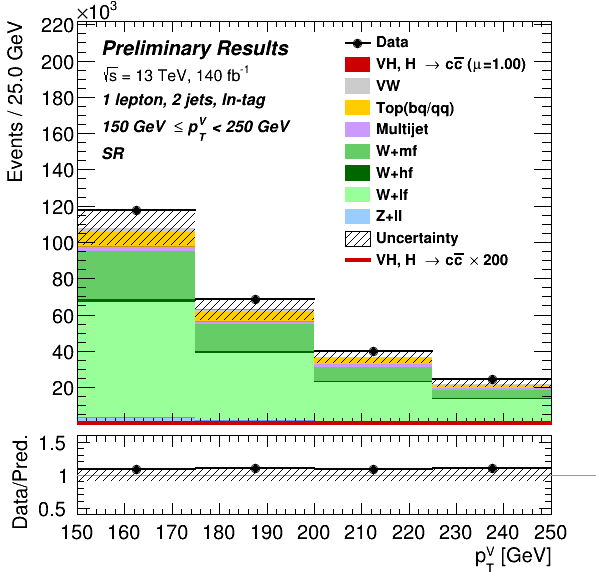
\includegraphics[width=\textwidth]{Images/VH/Own_fit/prefit_VHcc/Region_distpTV_BMax250_BMin150_DSR_J2_TTypeln_T1_L1_Y6051_Prefit.png}
      \caption{1-lepton $V+l$ CR $LN$.}
      \label{fig:plots_VHcc_ex_1L_CRvl}
  \end{subfigure}
  \begin{subfigure}[b]{0.32\textwidth}
    \centering
    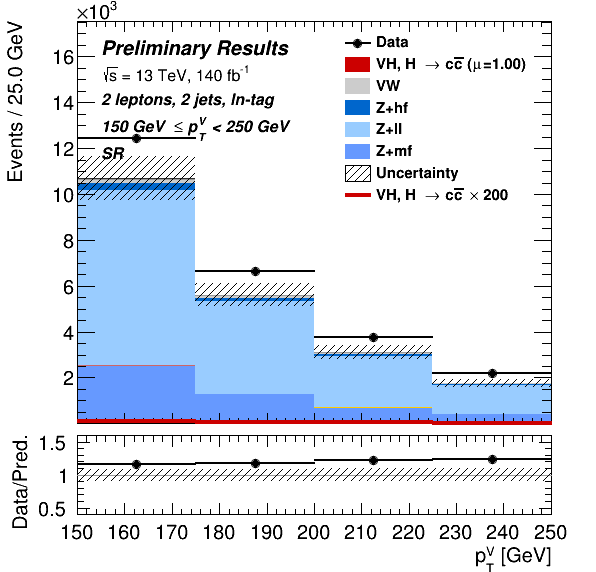
\includegraphics[width=\textwidth]{Images/VH/Own_fit/prefit_VHcc/Region_distpTV_BMax250_BMin150_DSR_J2_TTypeln_T1_L2_Y6051_Prefit.png}
    \caption{2-lepton $V+l$ CR $LN$.}
    \label{fig:plots_VHcc_ex_2L_CRvl}
\end{subfigure}
  \caption{A $BB$-tagged \lowdr\ CR (left - mvaCRLow distribution) and 2 $LN$-tagged $V+l$ CRs (centre and right - \ptv\ distributions), both with 2 jets and 150 GeV < \ptv\ < 250 GeV.}
  \label{fig:plots_VH_ex_CRL_CRvl}
\end{figure} 

\paragraph{$\boldsymbol{V +}$ light-jets Control Regions:} the $V +$ light-jets background is particularly significant for \vhc, due to the difficulties in discriminating $c$-jets from light-jets. Dedicated \glspl{cr}, called \textit{$V+l$ \glspl{cr}}, in the 1L and 2L channels target the \wlf\ and \zlf\ backgrounds\footnote{\vlf\ is a grouping of the $V+$jets with light-jets, introduced in Section~\ref{sec-modVjet}.}. They are defined by requiring exactly one loose $L$-tag $c$-jet without any $T$- nor $B$-tagged jet in the event. The selection is otherwise similar to that of the 1 $c$-tagged signal regions\footnote{Similarly to these SRs, there is no 1L $V+l$ CR for 75 GeV $<$ \ptv\ $<$ 150 GeV.}, with the candidate pair now tagged as $LN$, where $N$ is the leading untagged central jet. The 1L $V+l$ \glspl{cr} are 60\% pure in \wlf, while the 2L $V+l$ \glspl{cr} reach a 70\% \zlf\ purity. Two examples of kinematic distributions, for the 1L $V+l$ \glspl{cr} and 2L $V+l$ \gls{cr}, are shown in Figures~\ref{fig:plots_VHcc_ex_1L_CRvl} and \ref{fig:plots_VHcc_ex_2L_CRvl}, respectively. 

\subsubsection{Boosted Regime Categorisation}
In the boosted \vhb, two \ptv\ bins are considered, at [400, 600] GeV and $\geq$ 600 GeV, to avoid any overlap with the resolved \vhb. The \glspl{sr} are defined by requiring exactly 2 of the at most 3 leading track-jets associated with a single leading large-$R$ jet to be $b$-tagged, with no additional $B$-tagged track-jet outside the large-$R$ jet to enhance the top background rejection. All boosted regions, with processes normalised to their postfit expectations, are presented in Appendix Section~\ref{appsec-vh-analRegPosfit}. Figure~\ref{fig:plots_VHboost_ex} displays some signal regions, with the \glspl{sr} further separated into a high- (HP) and low-purity (LP) \glspl{sr} when there are, respectively, 0 or $\geq$ 1 additional small-$R$ jet not associated to the Higgs candidate large-$R$ jet. The different purity regions are combined in the final fit.

\paragraph{Boosted Top Control Regions in 0L and 1L:} the \ttb\ process is the main background in the 0L and 1L lepton channels, where a $t$-quark decay is captured as a single large-$R$ jet merging the produced $b$ and a hadronically decaying $W$. Boosted top control regions are defined for these lepton channels by selecting events that have an additional $B$-tagged track-jet outside of the large-$R$ jet, based on a requirement on their angular separation \[\Delta R(\textrm{VR-track jet, large-}R\textrm{ jet}) > 1.\] The boosted top \glspl{cr} effectively capture the \ttb\ signature by identifying the $b$-quark from the other decaying $t$-quark in the \ttb\ pair, using the same 85\% $b$-tagging \gls{wp} as for the Higgs candidate selection. An example of a boosted top \gls{cr} region is displayed in Figure~\ref{fig:plots_VHboost_ex_1L_top}.\\

\begin{figure}[h!]
  \centering
  \begin{subfigure}[b]{0.32\textwidth}
      \centering
      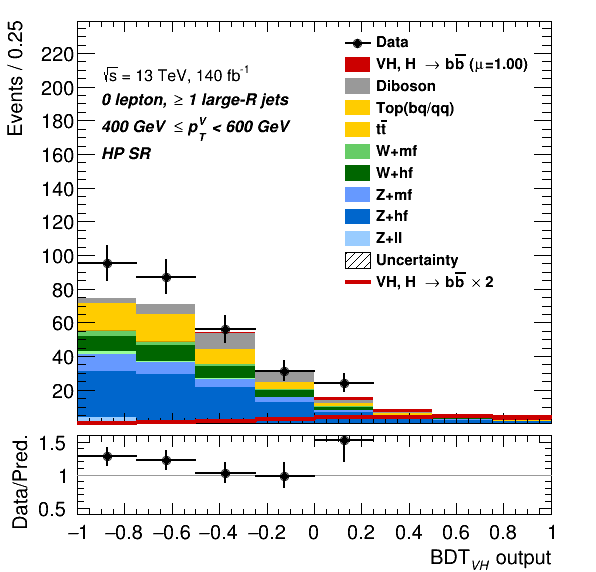
\includegraphics[width=\textwidth]{Images/VH/Own_fit/prefit_VHbb/Region_distmva_BMax600_BMin400_incFat1_Fat1_DSRnoaddbjetsr_J0_TTypebb_T2_L0_Y6051_Prefit.png}
      \caption{0-lepton high purity SR.}
      \label{fig:plots_VHboost_ex_0L_SR}
  \end{subfigure}
  \begin{subfigure}[b]{0.32\textwidth}
      \centering
      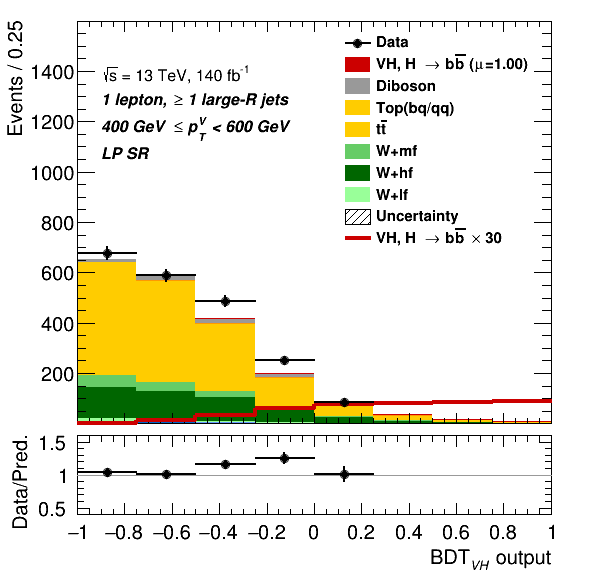
\includegraphics[width=\textwidth]{Images/VH/Own_fit/prefit_VHbb/Region_distmva_BMax600_BMin400_incFat1_Fat1_DSRnoaddbjetsr_J1_TTypebb_incJet1_T2_L1_Y6051_Prefit.png}
      \caption{1-lepton low purity SR.}
      \label{fig:plots_VHboost_ex_1L_SR}
  \end{subfigure}
  \begin{subfigure}[b]{0.32\textwidth}
    \centering
    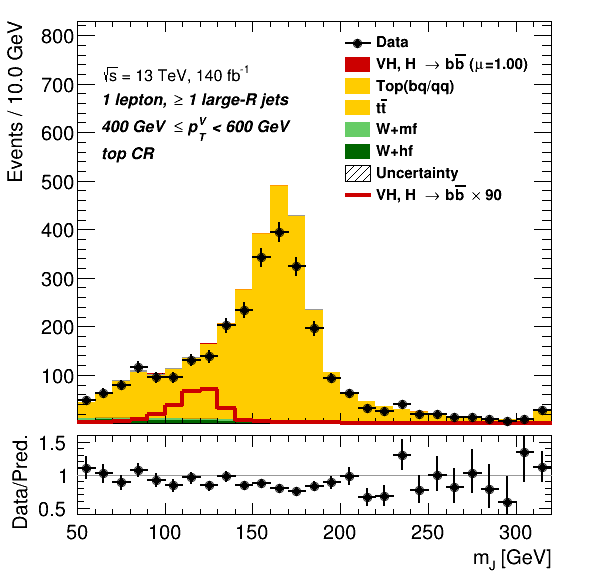
\includegraphics[width=\textwidth]{Images/VH/Own_fit/prefit_VHbb/Region_distmBB_BMax600_BMin400_incFat1_Fat1_DSRtopaddbjetcr_J0_TTypebb_incJet1_T2_L1_Y6051_Prefit.png}
    \caption{1-lepton top CR.}
    \label{fig:plots_VHboost_ex_1L_top}
\end{subfigure}
  \caption{Boosted $BB$-tagged signal regions \gls{bdt} distributions (left and centre) and boosted top CR $m_J$ distribution (right), with 400 GeV < \ptv\ < 600 GeV.}
  \label{fig:plots_VHboost_ex}
\end{figure} 

\subsection{Tagged-jets Corrections}\label{sec-vh-jetcor}
Several corrections to the energy of tagged jets are applied to improve the mass determination of the Higgs candidate. All jets benefit from the standard jet energy calibration introduced in Section~\ref{sec-atlas-jets}. Additional correction for $b$- and $c$-jets, summarised in Table~\ref{tab:bjetcorrectionregions}, leverage the unique properties of these heavy-flavour jets. The effects of the different reconstruction techniques are illustrated in Figure~\ref{fig:CorrResults} for inclusive 2-lepton invariant mass distributions in the different regimes of the analysis. \\

\begin{table}[!htbp]
  \begin{center}
  \resizebox{\textwidth}{!}{
    \begin{tabular}{c|c|cccc} \hline \hline
      Scheme & Lepton channel & Muon-in-jet & $P_T$-reco & Kinematic fit & \gls{fsr} Recovery     \\
      \hline
        \multirow{3}{*}{Resolved \vhb} & 0L & \checkmark & \checkmark &    & \\
                                      & 1L & \checkmark & \checkmark &    & \\  
                                      & 2L & \checkmark & \checkmark (\nj\ $\geq$ 4) & \checkmark (\nj\ $\leq$ 3) & \checkmark (\nj\ $\leq$ 4) \\  
      \hline
        \multirow{3}{*}{\vhc} & 0L & \checkmark &  &    & \\
                                      & 1L & \checkmark &  &    & \\  
                                      & 2L & \checkmark &  & \checkmark (\nj\ $\leq$ 3) & \checkmark (\nj\ $\leq$ 4) \\  
      \hline
        \multirow{3}{*}{boosted \vhb}  & 0L & \checkmark &  &    & \\
                                      & 1L & \checkmark &  &    & \\  
                                      & 2L & \checkmark &  &  \checkmark  & \\  

      \hline \hline
    \end{tabular}
  }
  \caption{The different Higgs candidate jet energy corrections.} 
  \label{tab:bjetcorrectionregions}
  \end{center}
\end{table}
  
\begin{figure}[h!]
  %\hspace{-4.0cm}
  \centering
  \begin{subfigure}[b]{0.49\textwidth}
    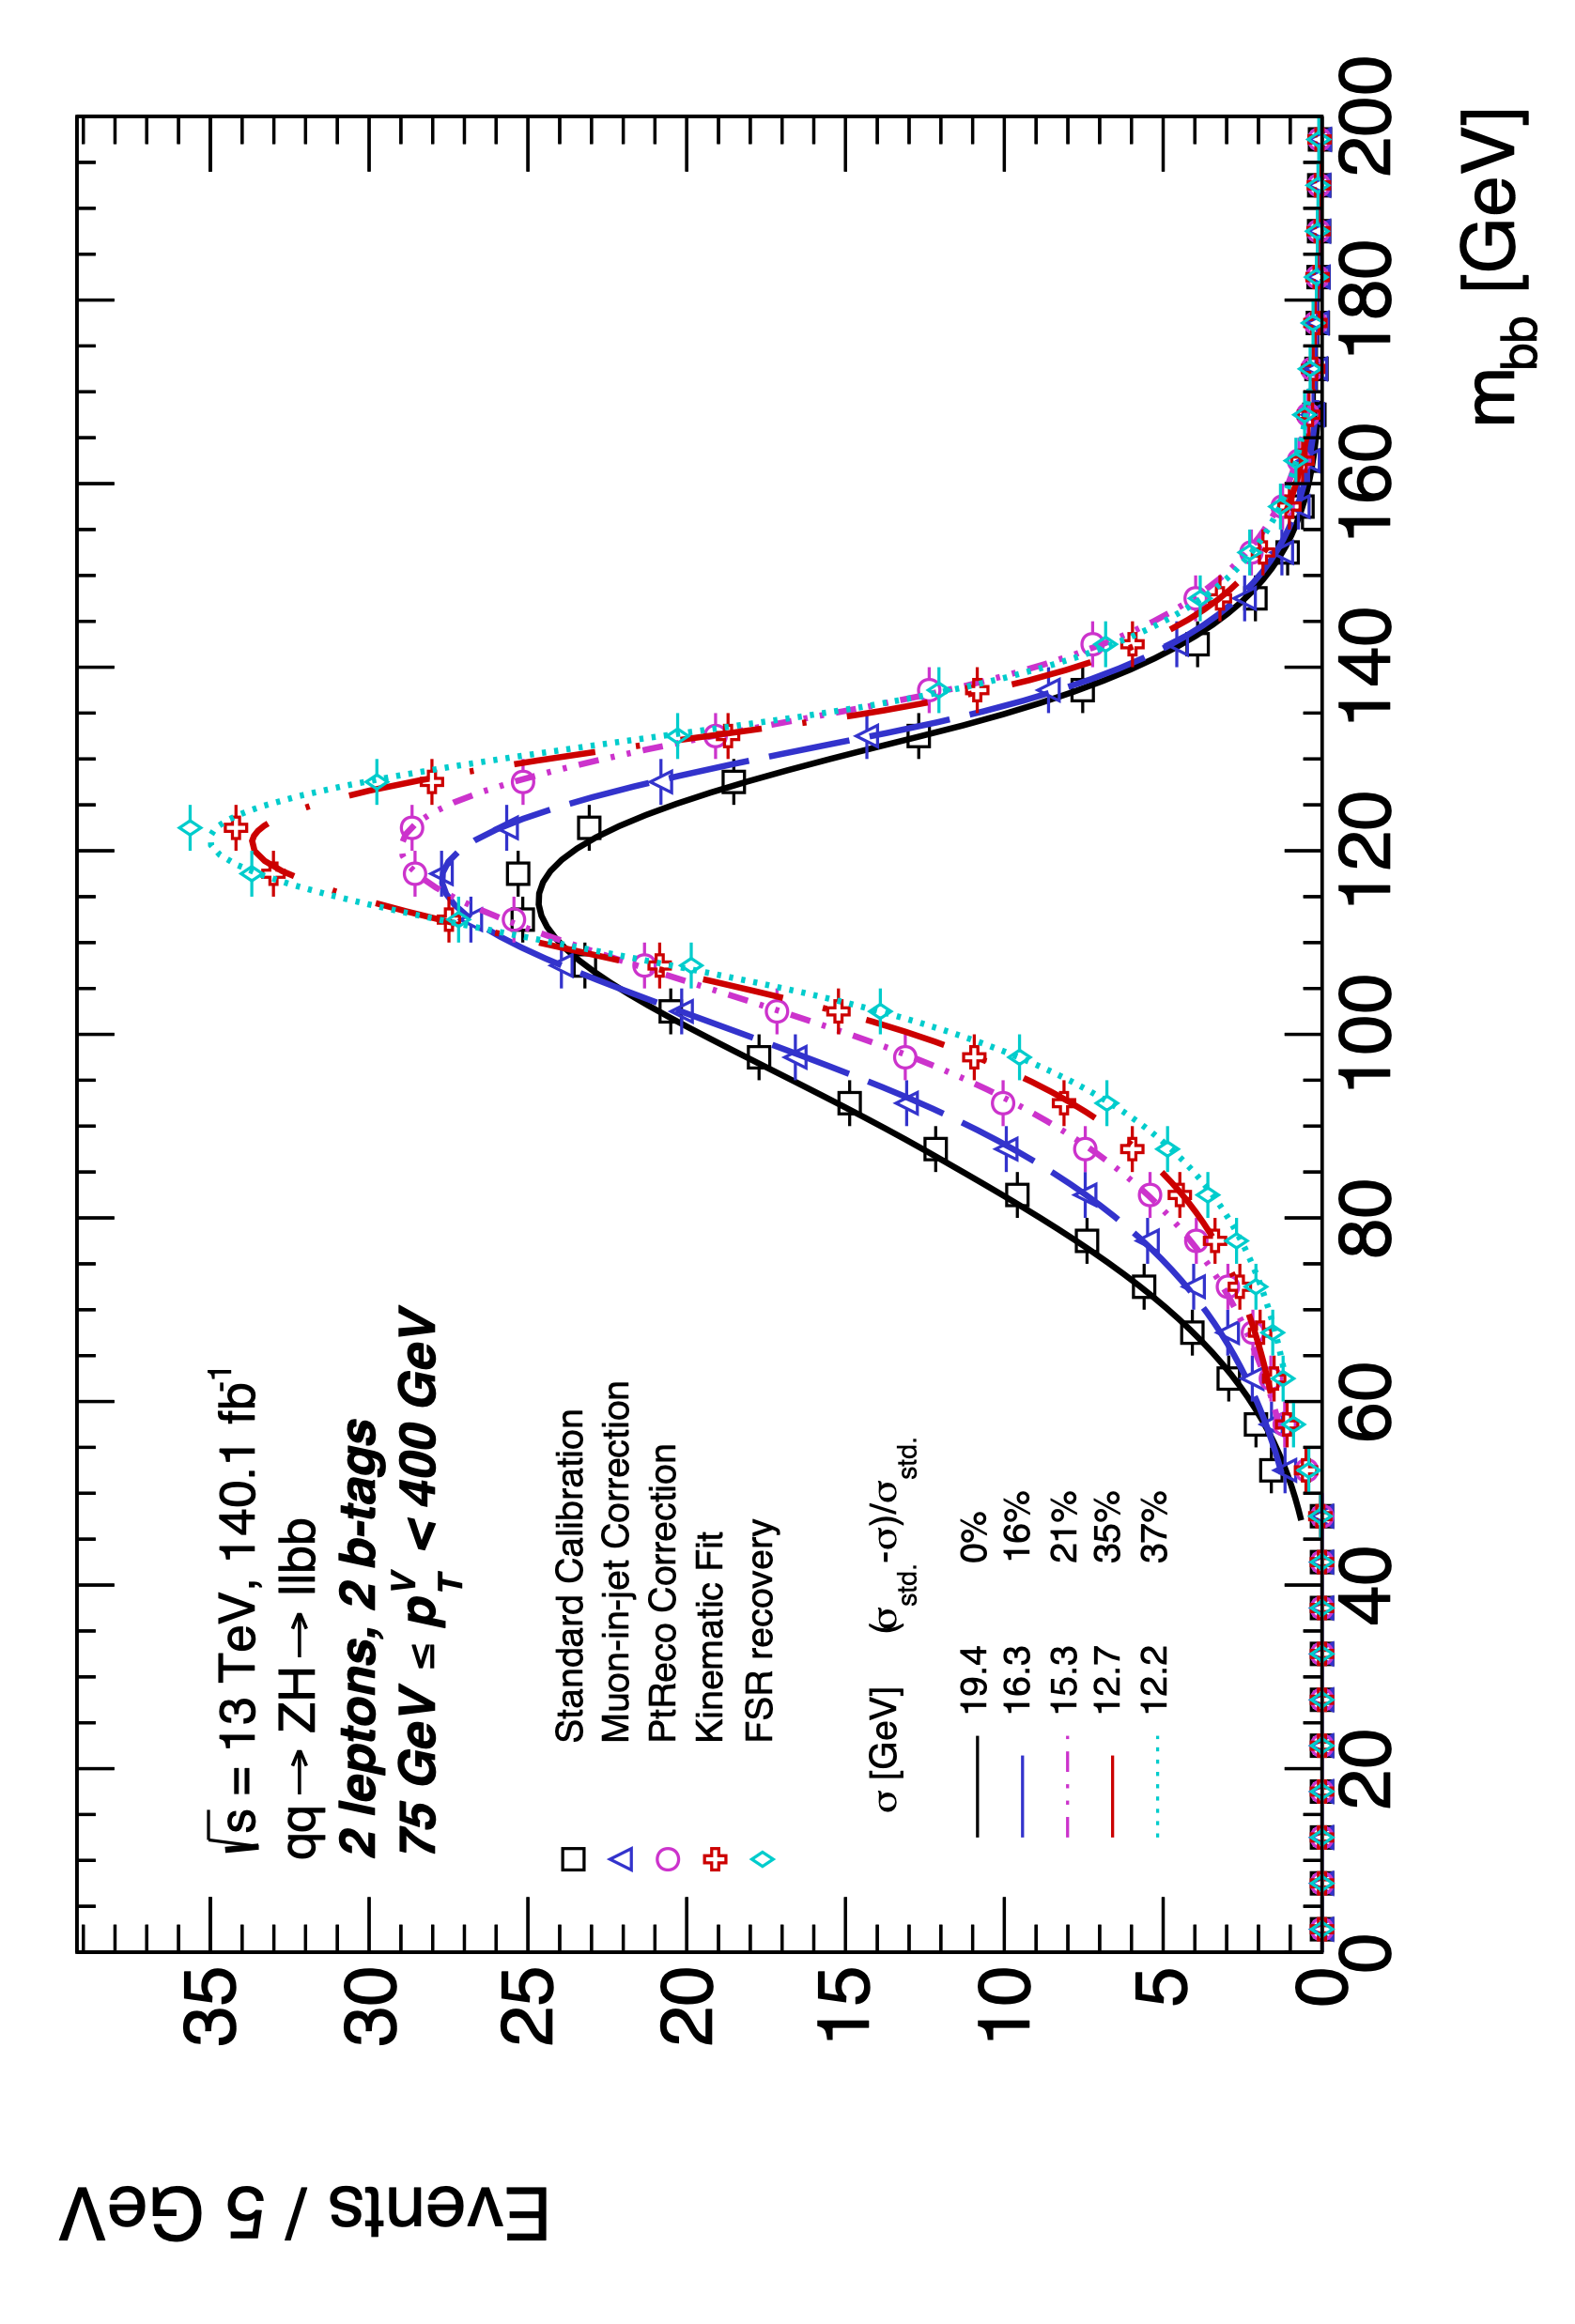
\includegraphics[width=\textwidth]{Images/VH/Correct/CorrectedDist/bbR.png}
  \caption{Resolved \vhb.} 
  \end{subfigure}
  \begin{subfigure}[b]{0.49\textwidth}
    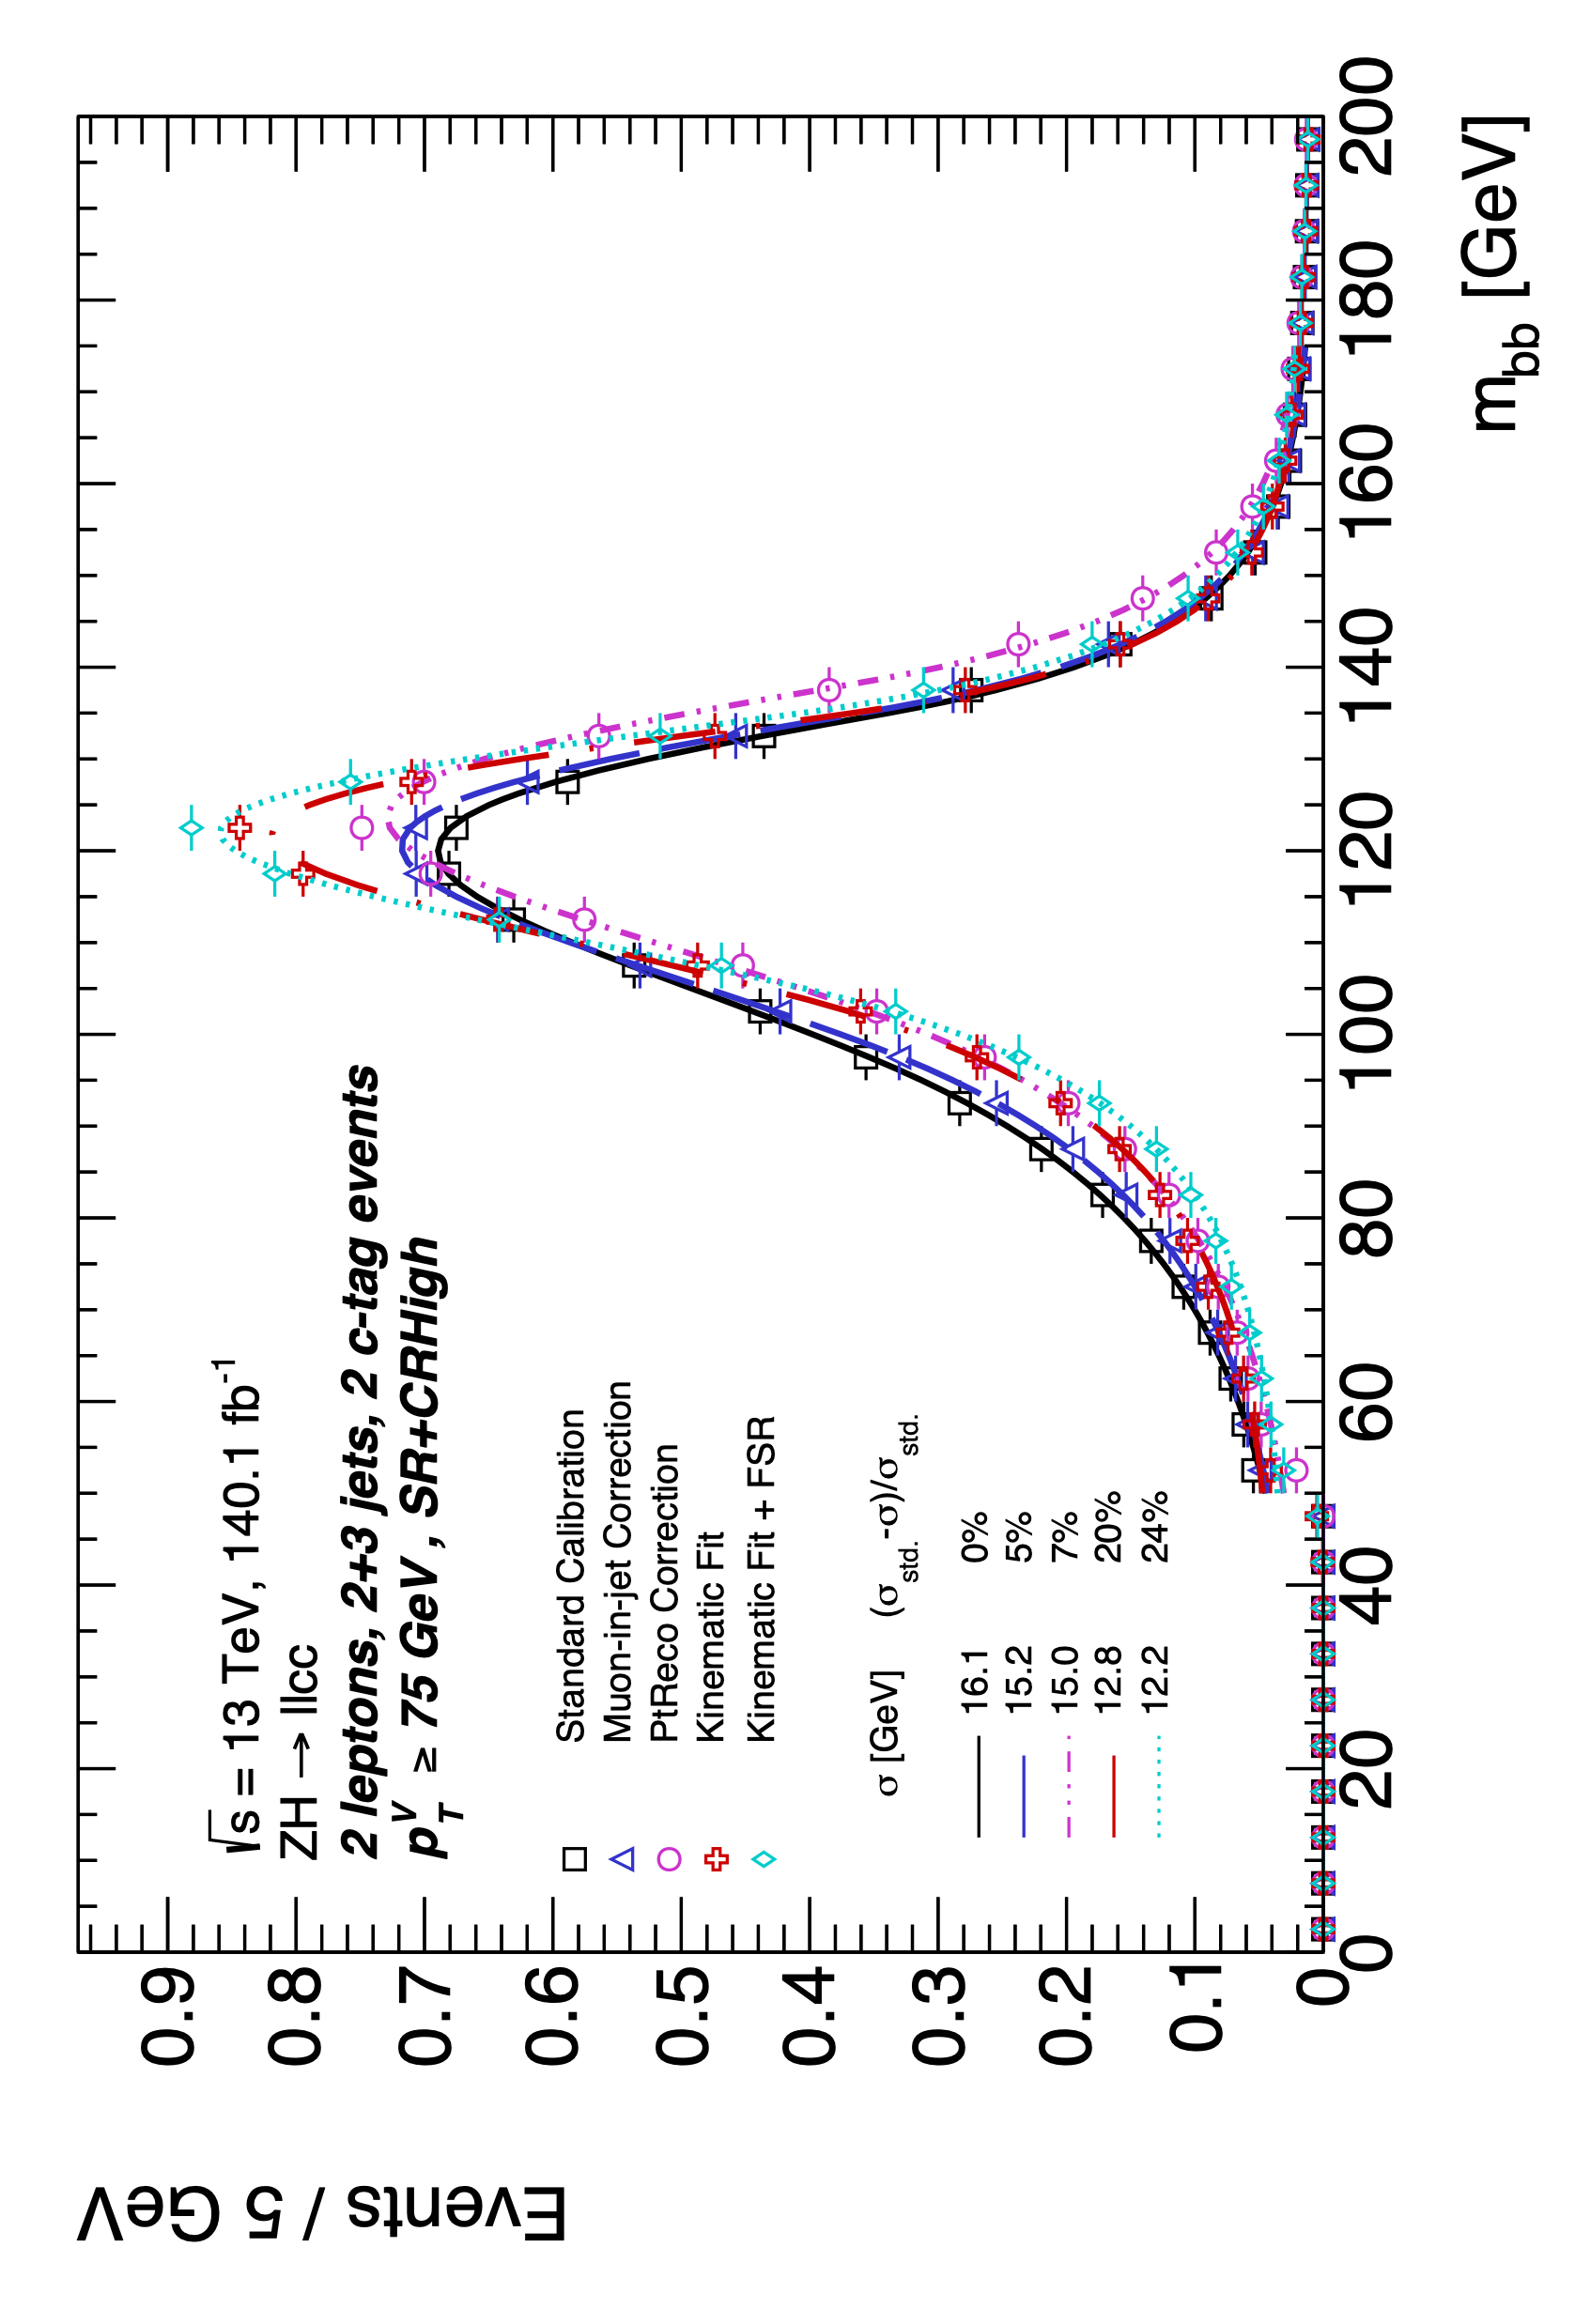
\includegraphics[width=\textwidth]{Images/VH/Correct/CorrectedDist/ccR.png}
    \caption{Resolved \vhc\ with 2 $c$-tags.}
  \end{subfigure} \\
  \begin{subfigure}[b]{0.49\textwidth}
    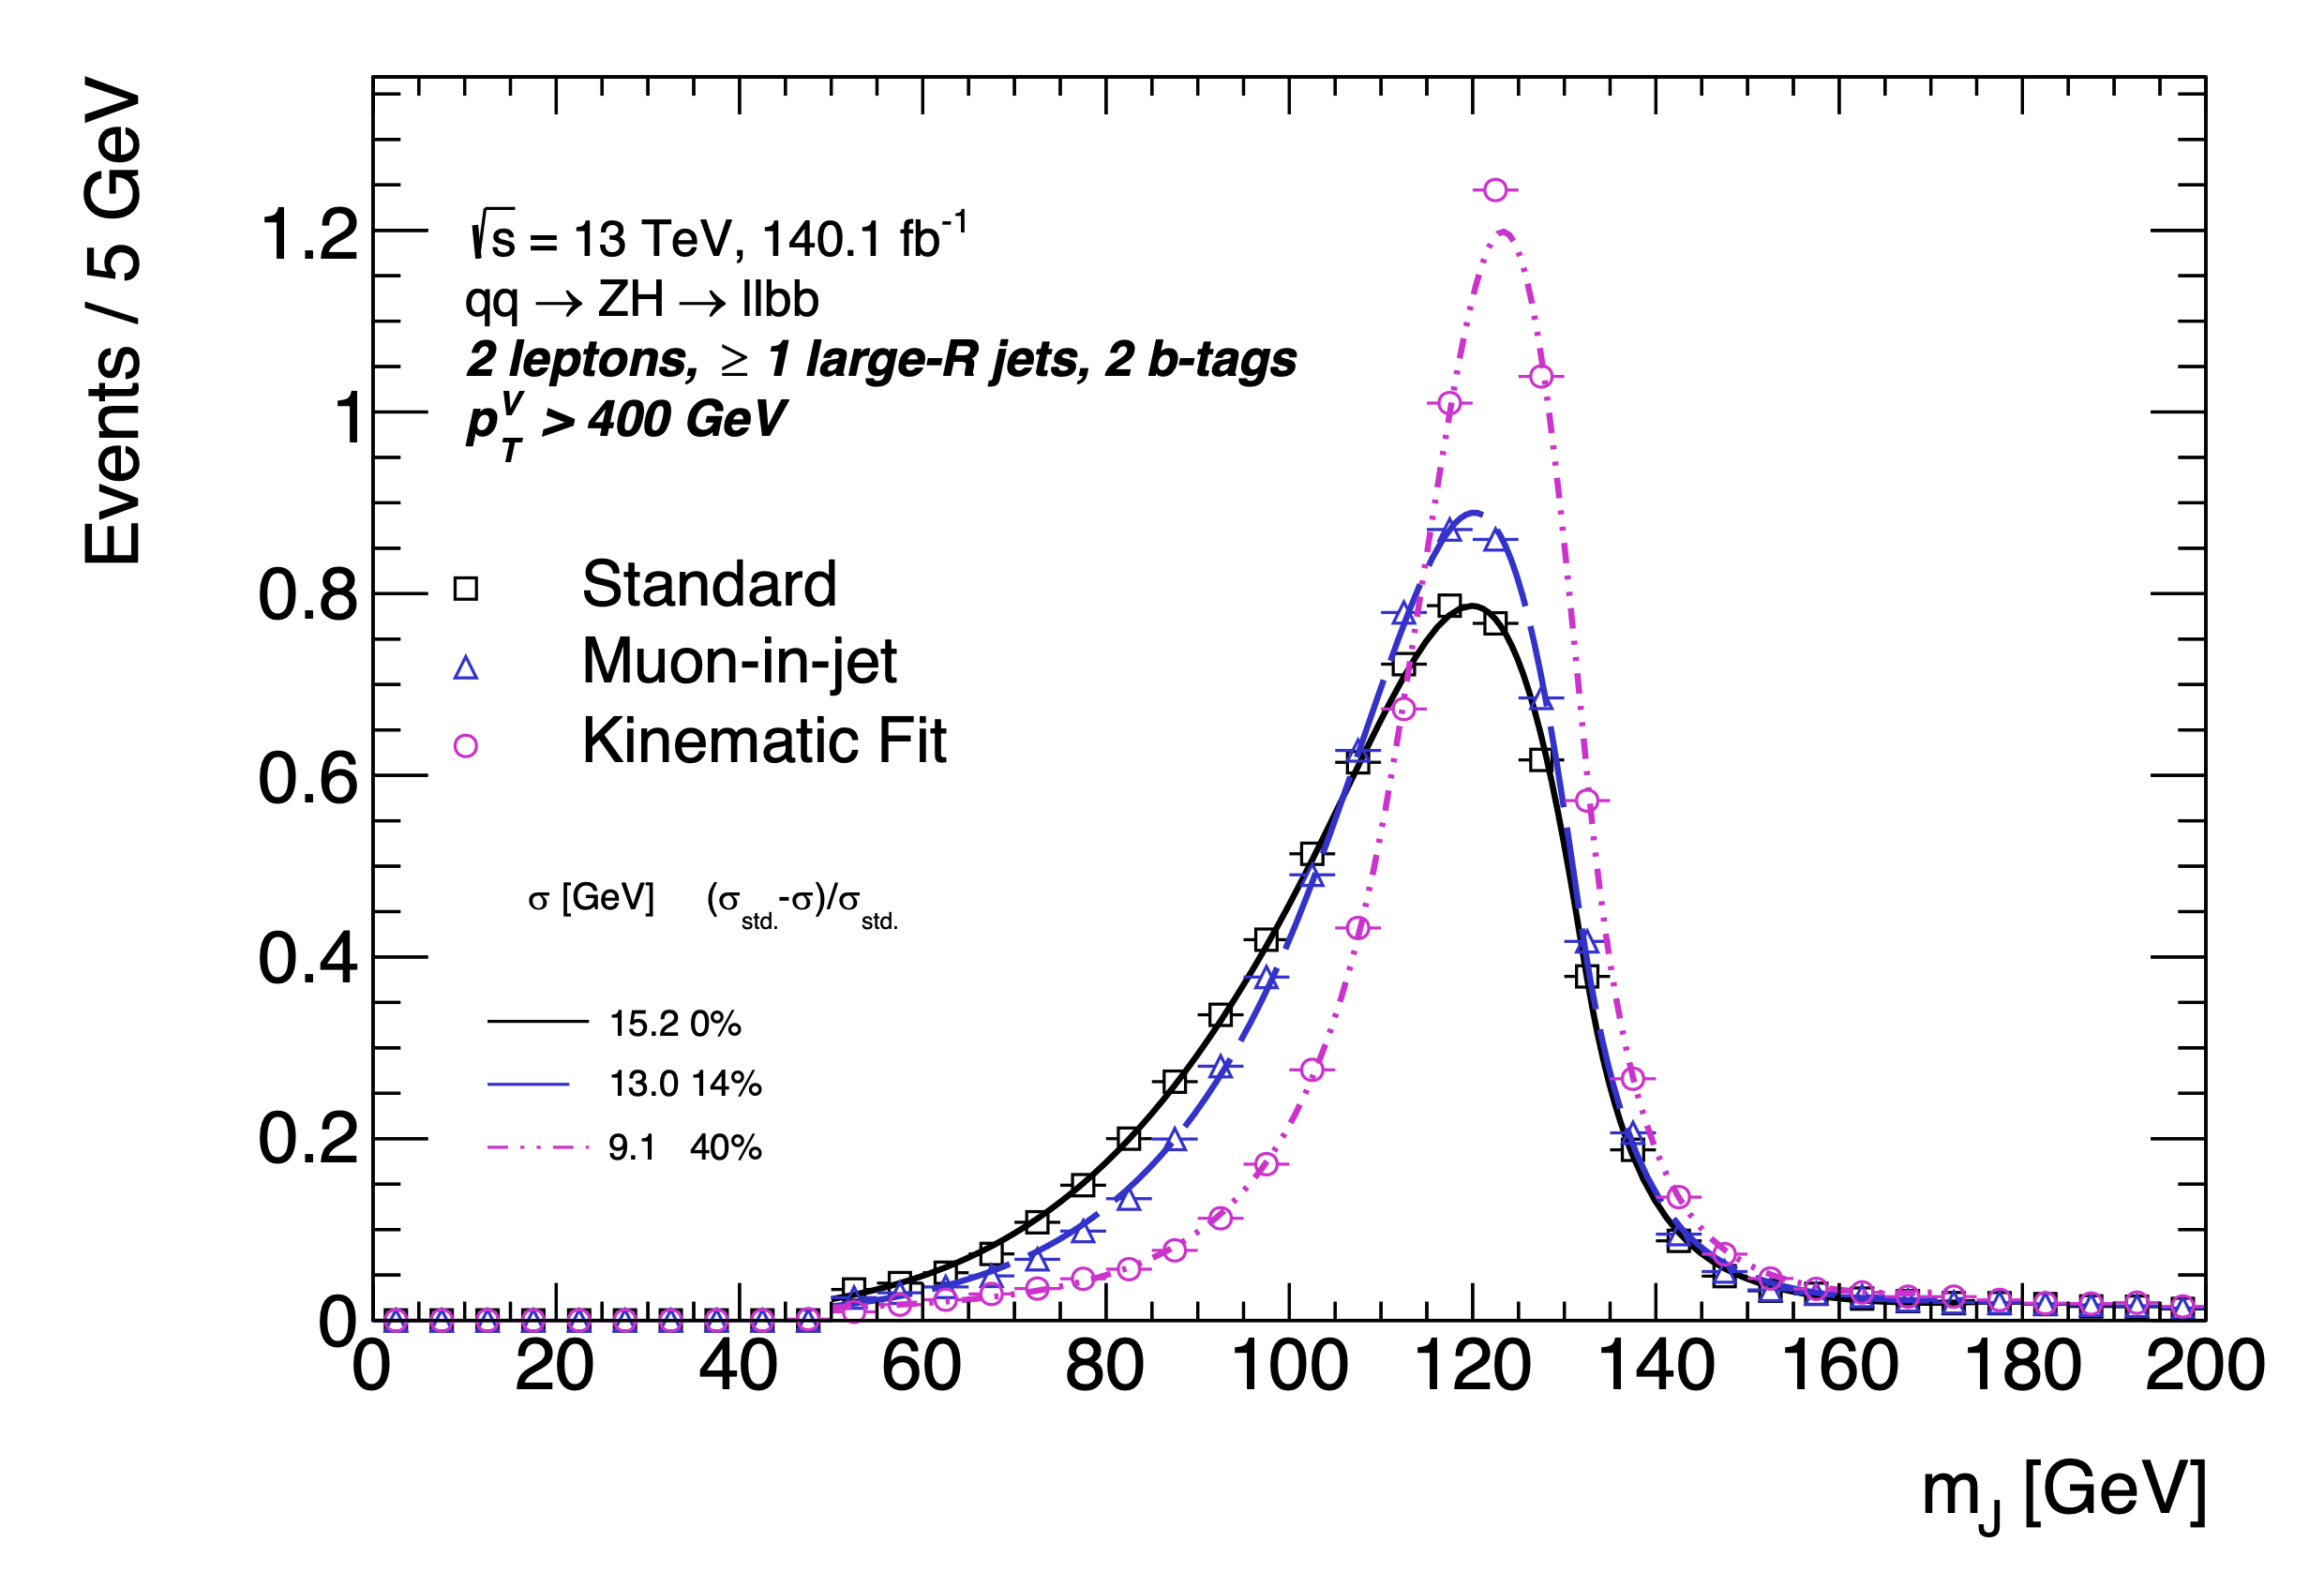
\includegraphics[width=\textwidth]{Images/VH/Correct/CorrectedDist/bbB.png}
    \caption{Boosted \vhb.}
  \end{subfigure}
  \caption{Distributions of the reconstructed Higgs candidate mass with the different jet corrections applied on simulated samples of the three analysis schemes in the 2-lepton channels, inclusive in \ptv\ and number of jets.}
  \label{fig:CorrResults}
\end{figure} 

\paragraph{\textit{Muon-in-jet} correction} is applied to all events to correct the energy of semi-leptonically decaying $b$- and $c$-jets with a muon in the jet cone. For the resolved regime, the closest muon 4-momentum $p_T^{\mu}$, as reconstructed from tracker information, is added to the jet if its angular separation from the jet axis respects \[\Delta R(\textrm{jet}, \mu) \leq \min\left(0.4, \,0.04 + \frac{10 \textrm{ GeV}}{p_T^{\mu}}\right).\] To avoid any double counting, the energy deposited by these muons in the calorimeter is subtracted from the muons 4-momenta, because it is already contributing to the jet energy. In the boosted scheme, the angular separation is measured with respect to the track-jets but the muon 4-momentum $p_T^{\mu}$ is added to the large-$R$ jet in case of a match.

\paragraph{\textit{$\boldsymbol{P_T}$-reco} correction} accounts for missing energy from neutrinos in the semi-leptonic decays and from the out-of-cone effect for $b$-jets. It is only applied to $b$-tagged jets in the resolved \vhb, across the the 0L and 1L channels and in the $\geq4$ jets 2L channel. The correction is derived from the signal samples of \vhb\ by comparing the truth jet $p_T$ and the reconstructed $p_T$ after the muon-in-jet correction. It is not applied to \vhc\ as it does not have a significant impact due to the lower likelihood of semi-leptonic decays and out-of-cone effects for $c$-jets.

\paragraph{\textit{Kinematic} fit correction} is applied in the 2L channel of the resolved regime, for events with 2 or 3 jets only. The $ZH \rightarrow \ell^+\ell^- b\bar{b} / \ell^+\ell^- c\bar{c}$ is fully reconstructed and a kinematic fit is applied to improve the $m_{jj}$ resolution after the previous corrections. The fit relies on a likelihood function with terms covering the object resolution, the jet transfer function, a $Z$ mass constraint, and system $p_T$ balance. The boosted 2L channel has a similar kinematic fit based on a Gaussian term. The procedure is not applied to events with more than 3 jets as the benefits are smeared out by the additional jets. % WARNING not clear for boosted. % NOTE not passed to the ETmiss.

\paragraph{FSR recovery} is deployed for events with 3 or 4 jets in the 2L resolved regime, to further improve the resolution of the $m_{bb}$ or $m_{cc}$ distributions after the kinematic fit correction. Such events are likely to have jets emanating as \glsreset{fsr}\gls{fsr}, whereby a quark or a gluon is emitted by a final state particle. A continuous cut on the sum $\Delta R_{j, j_1} + \Delta R_{j, j_2}$ of angular separations between a third or fourth jet ($j$) to the Higgs candidate jets ($j_1$ and $j_2$) is applied as a function of \ptv. Any additional jet below the cut is considered as a radiation and is added to the closest candidate jet. This effectively improves the reconstructed mass of Higgs bosons as well as the jet multiplicity, leading to an expected 7\% improvement in \vhb\ \gls{stxs} sensitivity by reducing the migration of events between measurement bins. This correction is not applied to 0L or 1L due to the possible increased acceptance of the \ttb\ background in the sensitive signal regions from the reduced jet multiplicty.